\chapter{Bifurcation Theory}

\subsection*{Section~\protect{\ref{S:TSPM}} Two Species Population Models}
\rhead{S:TSPM}{TWO SPECIES POPULATION MODELS}


\exer{c9.1.5}
\ans Predators eat prey faster in the first system \Ref{E:prpr1} than in 
the second system \Ref{E:prpr2}.

\soln  In the predator prey system \Ref{e:PP}, the $x$ variable is the
prey population and the $y$ variable is the predator population.  The
question asks: In which system will the predator population cause a
larger decrease in the prey population.  That is, in which system is
the coefficient $\sigma_1$ in \Ref{e:PP} a larger negative number?  In
the first system $\sigma_1=-10$, while in the second system $\sigma_1=-0.1$.

\exer{c9.1.6}   \ans  $\mu = 0.5$.

\soln  In the scaled system \Ref{e:PP2}, we found that
$\mu=|\mu_1/\mu_2|= |2/(-4)|=0.5$ for both systems \Ref{E:prpr1} and 
\Ref{E:prpr2}.  The scaling coefficients are given by \Ref{E:scalingcoeff}. 
For these systems $\gamma=-1/\mu_2=0.25$ and
$\alpha=\gamma\sigma_2=0.25$.  In the first system
$\beta=-\gamma\sigma_1= 2.5$ and in the second system $\beta=0.025$.

\exer{c9.1.2}
\ans For $\mu = 6$, there is a center at $e_4 = (1,8)$.

\soln First compute the equilibria for general $\mu$ by solving
$\dot{x} = \dot{y} = 0$.  The equilibria of the system occur at
$e_1 = (0,0)$, $e_2 = (0,4)$, $e_3 = (-\frac{\mu}{2},0)$, and
$e_4 = (\frac{\mu}{2} - 2, 2\mu - 4)$.  A center occurs at an equilibrium
where the Jacobian has purely imaginary eigenvalues; that is, where
$\trace{(dJ)} = 0$ and $\det{(dJ)} > 0$.  The general Jacobian of this
system is
\[
(dJ)_{(x,y)} = \cmattwo{\mu + 4x - y}{-x}{y}{1 + x - 0.5y}.
\]
At the equilibria,
\[
(dJ)_{e_1} = \mattwo{\mu}{0}{0}{1}, \quad
(dJ)_{e_2} = \cmattwo{\mu - 4}{0}{4}{-1}, \quad
\]
\[
(dJ)_{e_3} = \cmattwo{-\mu}{\frac{\mu}{2}}{0}{1 - \frac{\mu}{2}}, \quad
(dJ)_{e_4} = \cmattwo{\mu - 4}{2 - \frac{\mu}{2}}{2\mu - 4}{1 -
\frac{\mu}{2}}.
\]
For each of these matrices, find $\mu$ such that $\trace{(dJ)} = 0$.  At
$e_1$, $e_2$, and $e_3$, when $\trace{(dJ)} = 0$, $\det{(dJ)} < 0$.
At $e_4$, solve $\trace(dJ) = 0$ to obtain $\mu = 6$.  Then $\det{(dJ)}
= 4 > 0$; so the point $(1,8)$ is a center when $\mu = 6$.

\exer{c9.1.1}
(a) \ans See Table~\ref{c9.1.1}
\begin{table}[htb]
\begin{center}
\begin{tabular}{|c|c|c|c|}
\hline
& Exists in $1^{st}$ & Jacobian & equilibrium \\
& Quadrant & & type \\
\hline
$e_1 = (0,0)$ & always & $\mattwo{\mu}{0}{0}{1}$ & nodal source \\
\hline
$e_2 = \left(-\frac{\mu}{\rho},0\right)$ & always &
$\cmattwo{-\mu}{\frac{\mu}{\rho}}{0}{1 - \frac{\mu}{\rho}}$ &
saddle point \\
\hline
$e_3 = \left(0,-\frac{1}{\eta}\right)$ & always &
$\cmattwo{\mu + \frac{1}{\eta}}{0}{-\frac{1}{\eta}}{-1}$ &
$\begin{array}{c} \hbox{nodal sink if } \mu < -\frac{1}{\eta} \\
\hbox{saddle node if } \mu = -\frac{1}{\eta} \\
\hbox{saddle if } \mu > -\frac{1}{\eta} \end{array}$ \\
\hline
$\begin{array}{rl} e_4 = & (x_4,y_4) \\
 = & \dps\frac{1}{1 + \rho\eta}(-1 - \mu\eta, \mu - \rho) \end{array}$ 
& $\mu > -\frac{1}{\eta}$ &
$\cmattwo{\rho x_4}{-x_4}{y_4}{\eta y_4}$ & sink \\
\hline
\end{tabular}

\vspace{0.2in}
Table~\ref{c9.1.1}
\end{center}
\end{table}

\soln
Solve
\[
\begin{array}{rcccl}
\dot{x} & = & x(\mu + \rho x - y) & = & 0 \\
\dot{y} & = & y(1 + x + \eta y) & = & 0 \end{array}
\]
There are four solutions:
\[
\begin{array}{lr}
x = y = 0 & (e_1) \\
x \neq 0, y = 0 & (e_2) \\
x = 0, y \neq 0 & (e_3) \\
x \neq 0, y \neq 0 & (e_4) \end{array}
\]

Find the Jacobian matrices at these equilibria, which are shown in
Table~\ref{c9.1.1}.  To find the Jacobian at $e_4$, note that
$\mu + \rho x_4 - y_4 = 0$ and $1 + x_4 + \eta y_4 = 0$.  Therefore,
\[
(dJ)_{e_4} = \cmattwo{\mu + 2\rho x_4 - y_4}{-x_4}{y_4}{1 + x_4 +
2\eta y_4} = \cmattwo{\rho x_4}{-x_4}{y_4}{\eta y_4}.
\]

Use the Jacobian to find the type of each equilibrium.  Since $\mu > 0$,
both eigenvalues of $(dJ)_{e_1}$ are positive, so $e_1$ is a nodal source. 
Since $\det(dJ)_{e_2} < 0$, $e_2$ is a saddle point.  The trace of the
Jacobian at $e_3$ is always negative, so the equilibrium is a saddle if the
determinant is negative, a nodal sink if the determinant is positive, and
a saddle node if the determinant is zero.
For any valid $\rho$ and $\eta$, $\trace(dJ)_{e_4} = \rho x_4 +
\eta y_4 < 0$ and $\det(dJ)_{e_4} = x_4y_4(\rho\eta + 1) > 0$.
Define
\[
D = (\trace(dJ)_{e_4})^2 - 4\det(dJ)_{e_4} =
(\rho x_4 - \eta y_4)^2 - 4x_4y_4.
\]
Therefore, if $D > 0$, then $e_4$ is a spiral sink.  If $D = 0$, then
$e_4$ is an improper nodal sink, and if $D < 0$, then $e_4$ is a nodal
sink.

(b) If $e_4$ exists in the first quadrant, then all initial
populations such that $x > 0$ and $y > 0$ limit on $e_4$ in forward time. 
If $e_4$ does not exist in the first quadrant, then the population limits on
$e_3$, that is, the prey become extinct, and the population of predators
stabilizes at $-\frac{1}{\eta}$.  Figure~\ref{c9.1.1}a shows trajectories
of the system with $\mu = 2$, and Figure~\ref{c9.1.1}b shows trajectories
of the system with $\mu = 0.5$, so that $e_4$ no longer exists in the first
quadrant.

\begin{figure}[htb]
                       \centerline{%
                       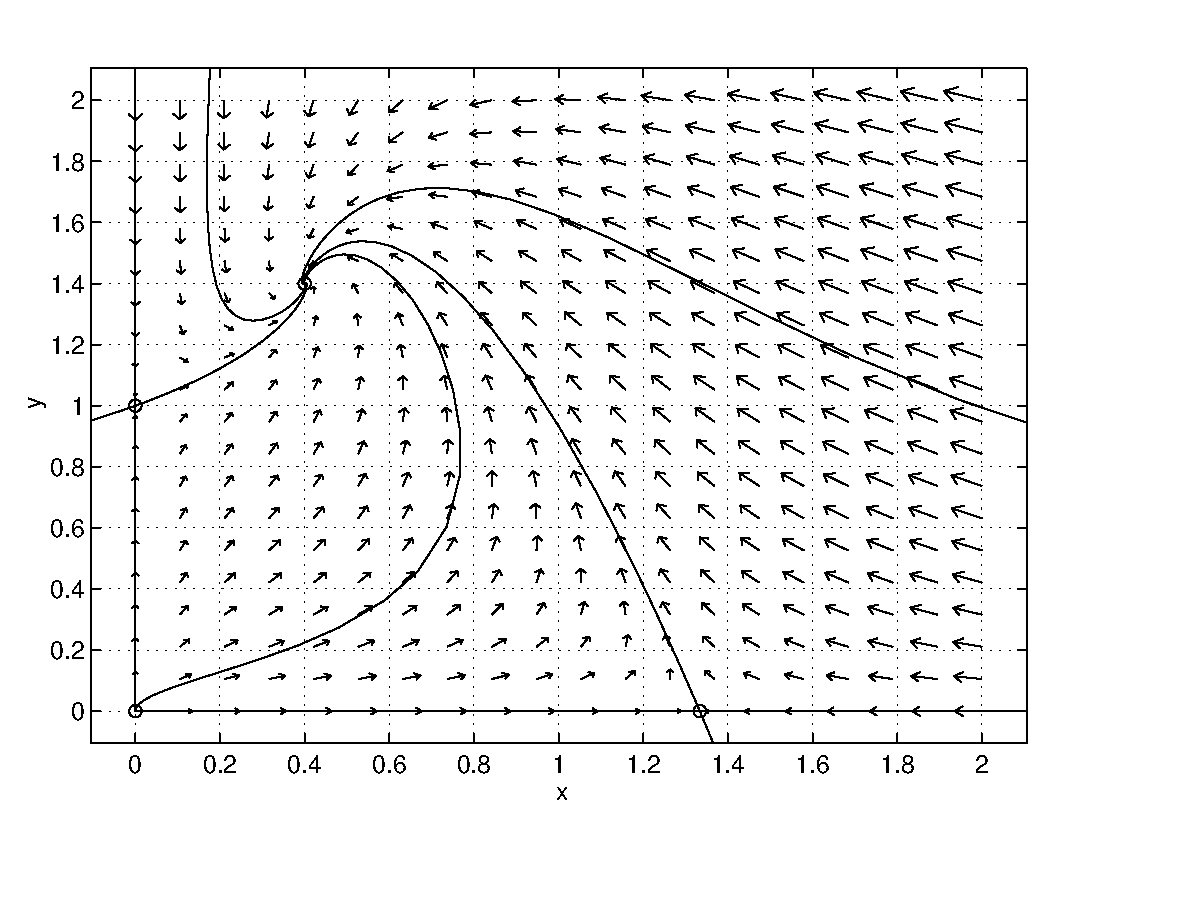
\psfig{file=exfigure/9-1-1a.eps,width=2.75in}
                       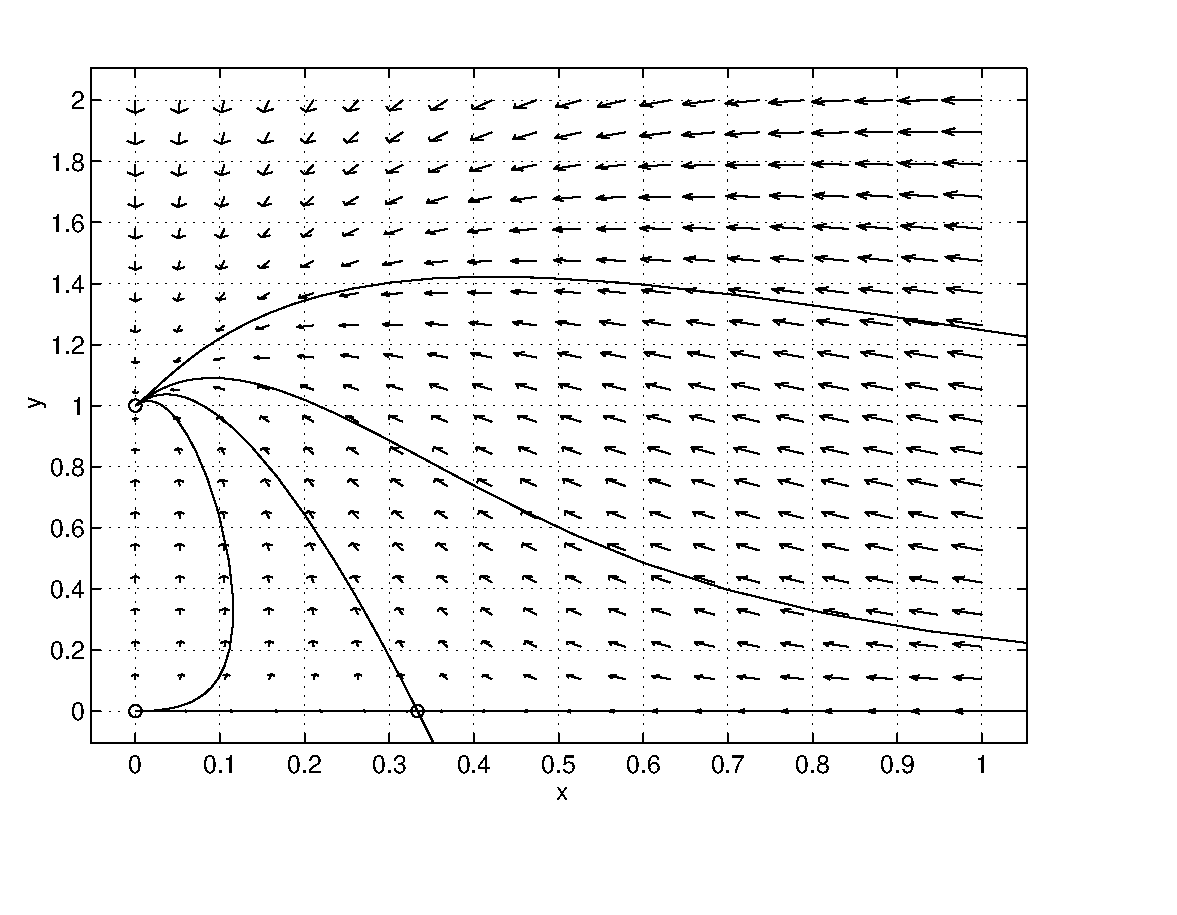
\psfig{file=exfigure/9-1-1b.eps,width=2.75in}}
                \exercaptwo{c9.1.1}
\end{figure}

\exer{c9.1.3}
Solve \Ref{e:PP} for $\dot{x} = \dot{y} = 0$ to find that there are
two equilibrium points, at $(0,0)$ and $(-\frac{\mu_2}{\sigma_2},
-\frac{\mu_1}{\sigma_1})$.  The second equilibrium is in the first
quadrant for any values of the constants that conform to the assumed
restrictions: $\mu_1 > 0$, $\mu_2 < 0$, $\sigma_1 < 0$, and
$\sigma_2 > 0$.  Load the system into {\tt pplane5} and graph with
several values for the constants to confirm that the nonzero
equilibrium is surrounded by periodic solutions.

\exer{c9.1.4}  Computer experiment.

\exer{c9.1.7}  Computer experiment.

\newpage
\exer{c9.1.8}
\ans (a) $\mu_1=\ln(2)$, $\mu_2=\ln(0.9)$, $\sigma_1 = -\frac{\ln(2)}{200}$,
and $\sigma_2 = -\frac{\ln(0.9)}{10000}$; (b) $86$ foxes; (c) 48,000 rabbits; 
(d) $10.5$ years.

\soln In the predator-prey equations $x$ denotes the prey population --- 
the rabbits --- and $y$ denotes the predator population --- the foxes.

\noindent (a) When $y=0$, the $\dot{x}$ equation can be solved for 
$x(t)=e^{\mu_1t}x_0$.  Thus when there are no foxes, the rabbit population 
doubles each year if $e^{\mu_1}=2$, that is, $\mu_1=\ln(2)$.  Similarly, when
$x=0$ the $\dot{y}$ equation can be solved for $y(t)=e^{\mu_2 t}y_0$.  So the
fox population decreases by 10\% each year in the absence of rabbits if 
$e^{\mu_2}=0.9$, that is, $\mu_2=\ln(0.9)$.

Next observe that there is just one equilibrium $(x_1,y_1)$ for the 
predator-prey equations when both populations are nonzero and that 
equilibrium is 
\[
(x_1,y_1) = \left(-\frac{\mu_2}{\sigma_2},-\frac{\mu_1}{\sigma_1}\right) = 
\left(-\frac{\ln(0.9)}{\sigma_2},-\frac{\ln(2)}{\sigma_1}\right) = 
(10000,200).
\]
So
\[
\sigma_1 = -\frac{\ln(2)}{200}<0 \quad \mbox{and} \quad
\sigma_2 = -\frac{\ln(0.9)}{10000}>0.
\]
Thus, under these conditions, the predator-prey model is:
\begin{equation}  \label{E:PPspec}
\begin{array}{rcl}
\dot{x} & = & x(\ln(2) - \ln(0.9)y/10000) \\
\dot{y} & = & y(\ln(0.9) - \ln(2)x/200),
\end{array}
\end{equation}

\noindent (b) Using the {\sf Keyboard input} button and the {\sf Specify a
computation interval} in that menu, we can compute the solution with initial
condition $(x_0,y_0)=(1200,110)$ until time $t=3$ years.  The result is that
the number of foxes is $86$ as can be seen from the time series in 
Figure~\ref{c9.1.8}a.

\noindent (c)  Using the {\sf Keyboard input} button, we can start
integrating the differential equation with initial condition
$(x_0,y_0)=(1200,110)$.  Graphing the $x$ time series (the rabbit population)
we get the result shown in Figure~\ref{c9.1.8}b.  Specifically, the 
maximum is approximately 48,000 rabbits. 

\noindent (d)  The maximum rabbit population occurs for the first time about 
$10.5$ years after the storm.

\begin{figure}[htb]
     \centerline{%
     \psfig{file=exfigure/PPinit2.eps,width=2.75in}
     \psfig{file=exfigure/PPinit.eps,width=2.75in}}
     \caption{(Left) Time series $y$ vs. $t$ of (\protect\ref{E:PPspec}) 
	showing population of foxes after three years. (Right) Time series $x$ 
	vs. $t$ of (\protect\ref{E:PPspec}) showing maximum rabbit population.}
     \exercaptwo{c9.1.8}
\end{figure}

\subsection*{Section~\protect{\ref{S:bifurcation}} Examples of Bifurcation}
\rhead{S:bifurcation}{EXAMPLES OF BIFURCATION}

\exer{c9.7.1}
\ans The bifurcation diagram (Figure~\ref{c9.7.1}) shows two equilibria
vanishing as $\rho$ increases through $0$.

\soln The equilibria of the equation occur when $0 = \frac{dx}{dt} =
\rho + x^2$; that is, when $\rho = -x^2$.  Thus, when $\rho < 0$, there
are two equilibria, at $x = \pm\sqrt{-\rho}$.  When $\rho = 0$, there is
one equilibrium at $x = 0$; and when $\rho > 0$, there are no real
equilibria.  Let $f(x,\rho) = \rho + x^2$.  If $\rho < 0$, 
then $f_x(\sqrt{-\rho},\rho) > 0$ and $f_x(-\sqrt{-\rho},\rho) < 0$. 
Thus, the equilibrium at $x = \sqrt{-\rho}$ is unstable, and the
equilibrium at $x = -\sqrt{-\rho}$ is stable.

\begin{figure}[htb]
                       \centerline{%
                       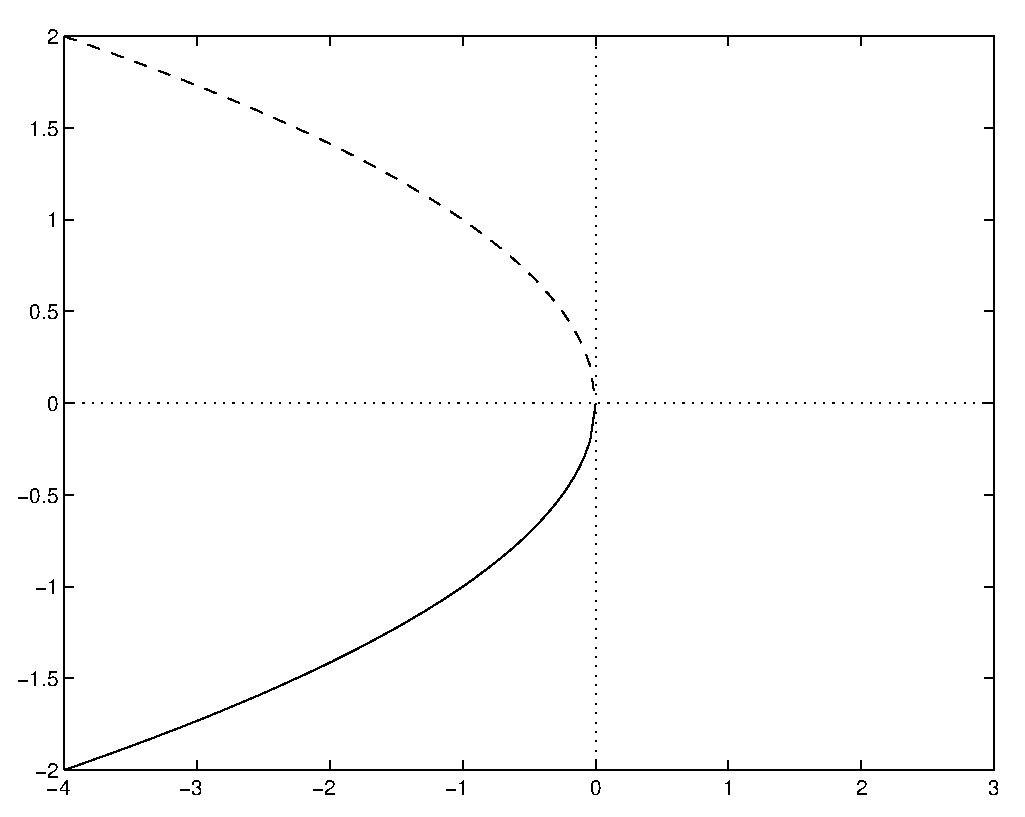
\psfig{file=exfigure/9-7-1.eps,width=3.0in}}
                \exercap{c9.7.1}
\end{figure}

\exer{c9.7.2}
\ans The bifurcation diagram (Figure~\ref{c9.7.2}) shows two equilibria
appearing as $\rho$ increases through $-1$.

\soln The equilibria of the equation occur when $f(x,\rho) = \rho - x^2 +
2x = 0$.  Solve for $x$ in this equation to find that $x = 1 \pm
\sqrt{\rho + 1}$ at all equilibria.  Thus, the differential equation has
two real equilibria when $\rho > -1$, one real equilibrium at $x = 1$ when
$\rho = -1$, and no real equilibria when $\rho < -1$.  To find the
stability of the equilibria, compute $f_x(x,\rho) = -2x + 2$.  Thus, if
$\rho > -1$, then
$f_x(1 + \sqrt{\rho + 1},\rho) = -2\sqrt{\rho + 1} < 0$ and
$f_x(1 - \sqrt{\rho + 1},\rho) = 2\sqrt{\rho + 1} > 0$.

\begin{figure}[htb]
                       \centerline{%
                       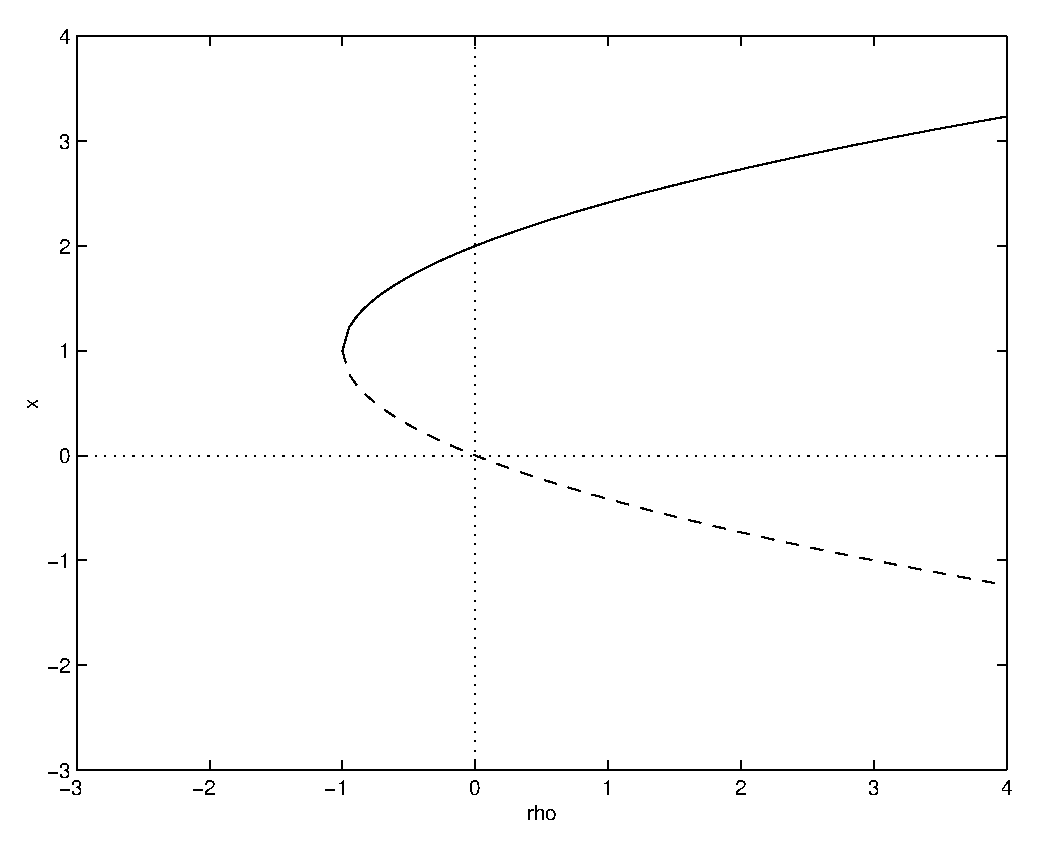
\psfig{file=exfigure/9-7-2.eps,width=3.0in}}
                \exercap{c9.7.2}
\end{figure}

\exer{c9.7.3}
\ans The maximum number of equilibria is 4.  This maximum occurs when
$8 < \rho < 13$.  The bifurcation diagram is shown in Figure~\ref{c9.7.3}.

\soln The equilibria of the equation occur when
$\rho = 3x^4 - 8x^3 - 6x^2 + 24x$.  Note that minimum and maximum points of
$\rho$ as a function of $x$ occur when $\rho_x = 0$.  Thus, minima occur
at $(x,\rho) = (-1,-19)$ and $(x,\rho) = (2,8)$, and a maximum occurs at
$(x,\rho) = (1,13)$.  So, as $\rho$ increases, two equilibria appear at
$\rho = -19$, two equilibria appear at $\rho = 8$, and two equilibria
disappear at $\rho = 13$.  When $x < -1$ and when $1 < x < 2$, equilibria
are stable.  For $-1 < x < 1$ and $2 < x$, equilibria are unstable.

\begin{figure}[htb]
                       \centerline{%
                       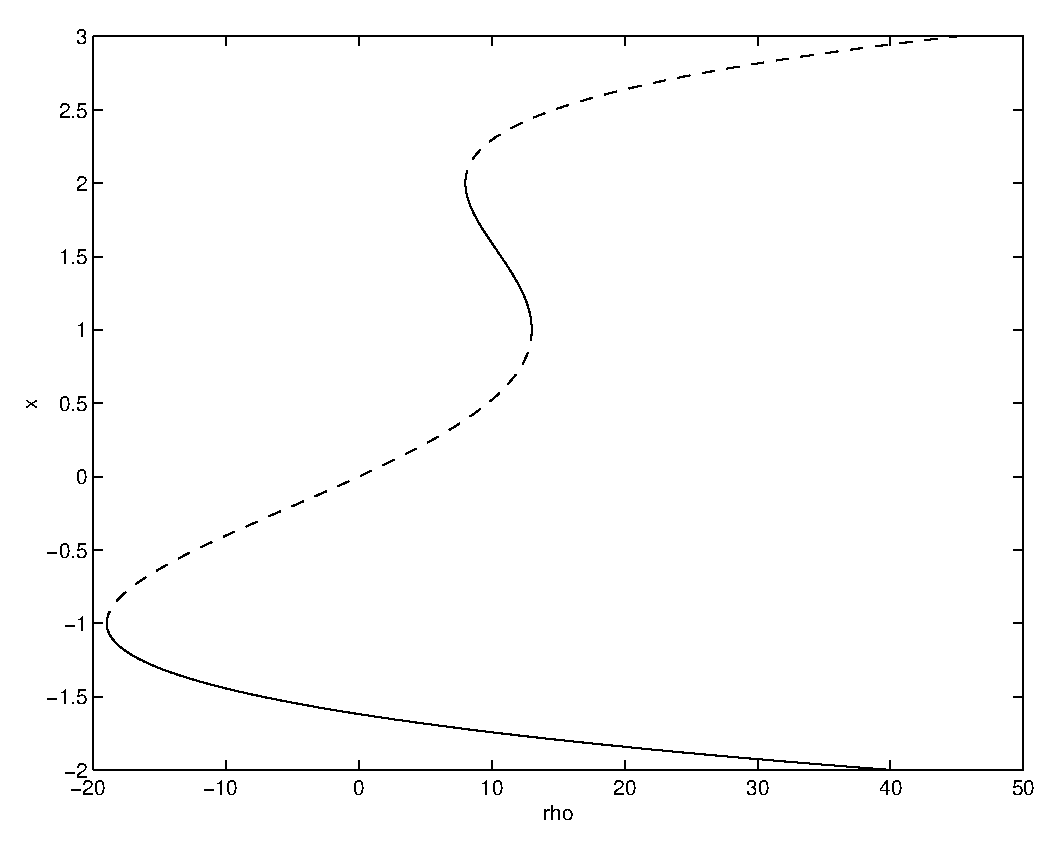
\psfig{file=exfigure/9-7-3.eps,width=3.0in}}
                \exercap{c9.7.3}
\end{figure}

\exer{c9.4.1}
Find equilibria in the Van der Pol equations by setting $\dot{y}=0$ 
to obtain $x=0$ and $\dot{x} = 0$ to obtain $y=0$.  This calculation
verifies that $(0,0)$ is the only equilibrium of the Van der Pol system.  

A Hopf bifurcation occurs at the equilibrium at the origin when 
the Jacobian at the origin has zero trace and positive determinant.  
The Jacobian of the Van der Pol system is
\[
J = (dJ)_{(0,0)} = \left.\cmattwo{\rho-3x^2}{-1}{1}{0}\right|_{(0,0)} =
\mattwo{\rho}{-1}{1}{0}.
\]
Thus, $\det(J) = 1 > 0$ and $\trace(J) = \rho$.  Hopf bifurcation can only
occur in this system when $\rho = 0$.  Figure~\ref{c9.4.1}a shows
a {\tt pplane5} graph of the system with $\rho = 0$, and
Figure~\ref{c9.4.1}b shows the system with $\rho = 0.4$.  One limit
cycle can be seen surrounding the origin in this graph.

\begin{figure}[htb]
                       \centerline{%
                       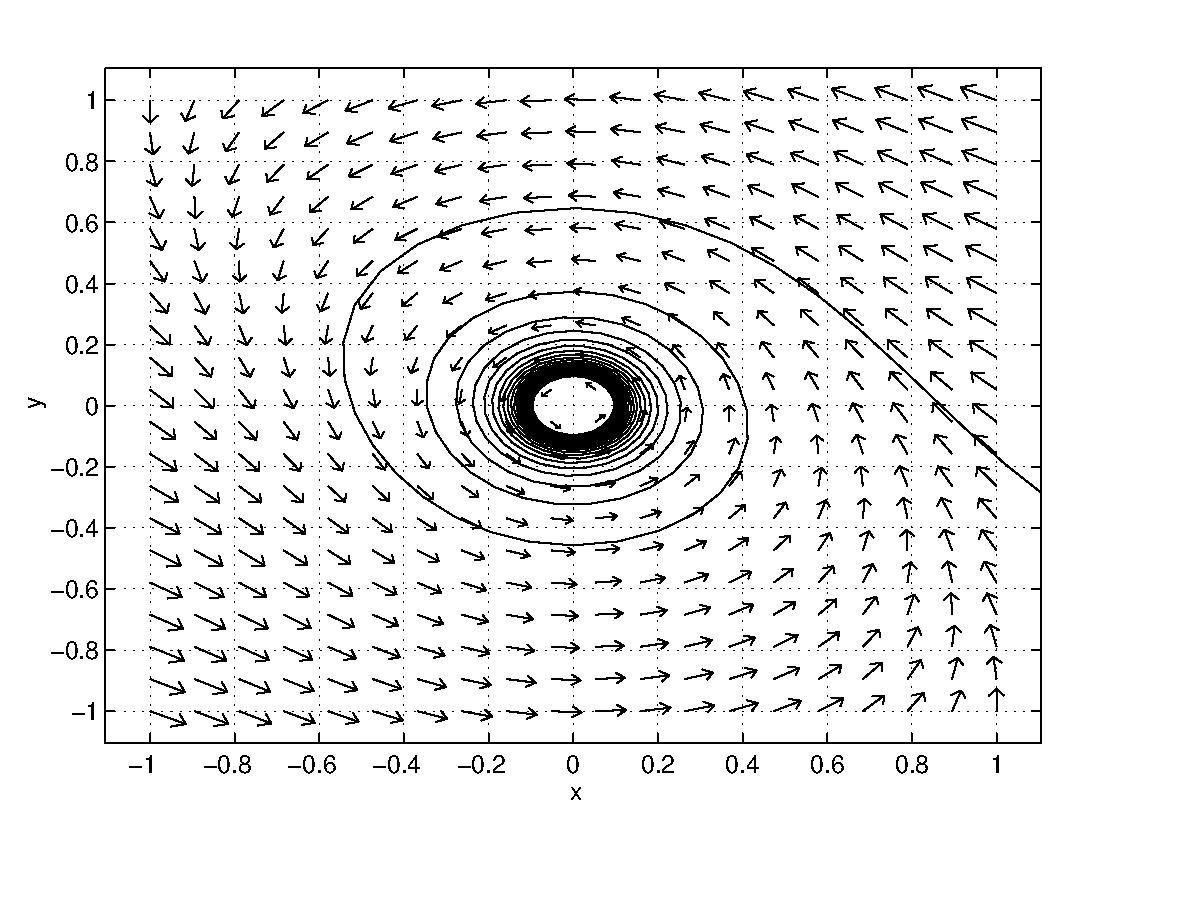
\psfig{file=exfigure/9-4-1a.eps,width=2.75in}
                       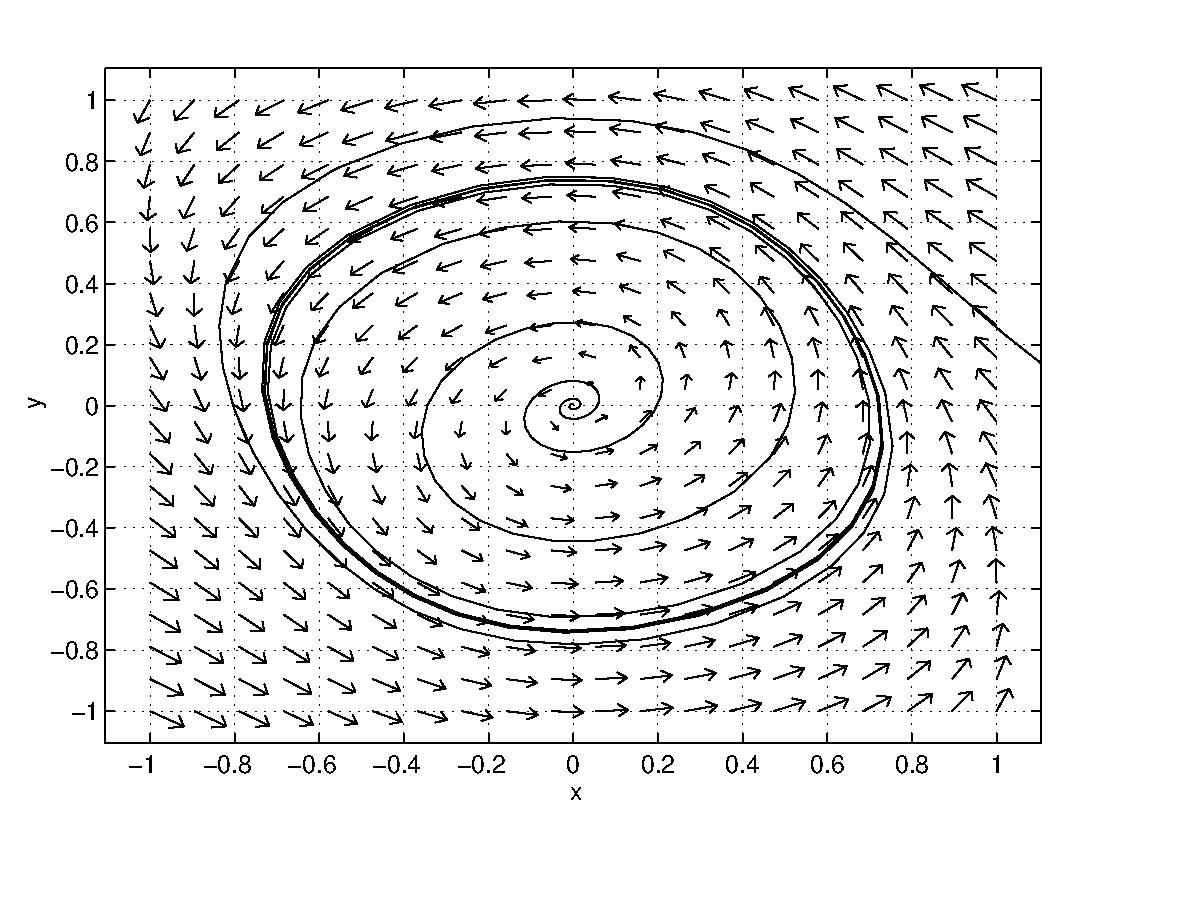
\psfig{file=exfigure/9-4-1b.eps,width=2.75in}}
                \exercaptwo{c9.4.1}
\end{figure}

\exer{c9.4.2}
\ans When $\rho = 0$, the differential equation can have a Hopf bifurcation 
only at $(x_0,y_0) = (2,1)$.

\soln A Hopf bifurcation can occur at an equilibrium point only when the 
trace of the Jacobian at this point is zero and the determinant of the 
Jacobian is positive.  In this case, the Jacobian of the differential 
equation at $\rho = 0$ is
\[
J_{(x,y)} = \mattwo{3 + 2x}{-4 - 4y}{14x - 3y}{-1 - 3x}.
\]
Then, $\trace(J_{(x,y)}) = 2 - x$; so $\trace(J) = 0$ when $x = 2$.  Solve
the differential equation for $\dot{x} = 0 = \dot{y}$ to find that $(x,y) =
(2,1)$ is an equilibrium point.  Since $\det(J_{(2,1)}) = 151 > 0$, this 
point can be a Hopf bifurcation point when $\rho = 0$.


\exer{e:source}
\ans When $\rho < 0$, neither system has an equilibrium.  All solutions of
this system limit on the negative $x$-axis in backwards time, while all
solutions of \Ref{E:ssys} limit on the positive $x$-axis in forward time.
When $\rho > 0$, each system has two equilibria along the $x$-axis.  This
system has a saddle at $x < 0$ and a source at $x > 0$, while \Ref{E:ssys}
has a saddle at $x > 0$ and a sink at $x < 0$.

\soln
A saddle node bifurcation can occur only when the Jacobian of a system
at an equilibrium has a zero eigenvalue.  The only equilibrium for this
system occurs at the point $(x,y) = (\pm\sqrt{\rho},0)$.  The Jacobian
at the point $(x,y) = (\sqrt{\rho},0)$ is
\[
J = \cmattwo{2\sqrt{\rho}}{1}{0}{\rho + 1}.
\]
The determinant of $J$ is zero only if $2\sqrt{\rho}(\rho + 1) = 0$, which
occurs when $\rho = 0$.  Thus, $\rho = 0$ is the only point at which a
saddle node bifurcation can occur.  The system is shown in
Figure~\ref{e:source}a with $\rho = -0.1$, and in Figure~\ref{e:source}b
with $\rho = 0.1$.  There are no equilibria when $\rho = -0.1$, and two
when $\rho = 0.1$, so there is indeed a saddle node bifurcation when
$\rho = 0$.

\begin{figure}[htb]
                       \centerline{%
                       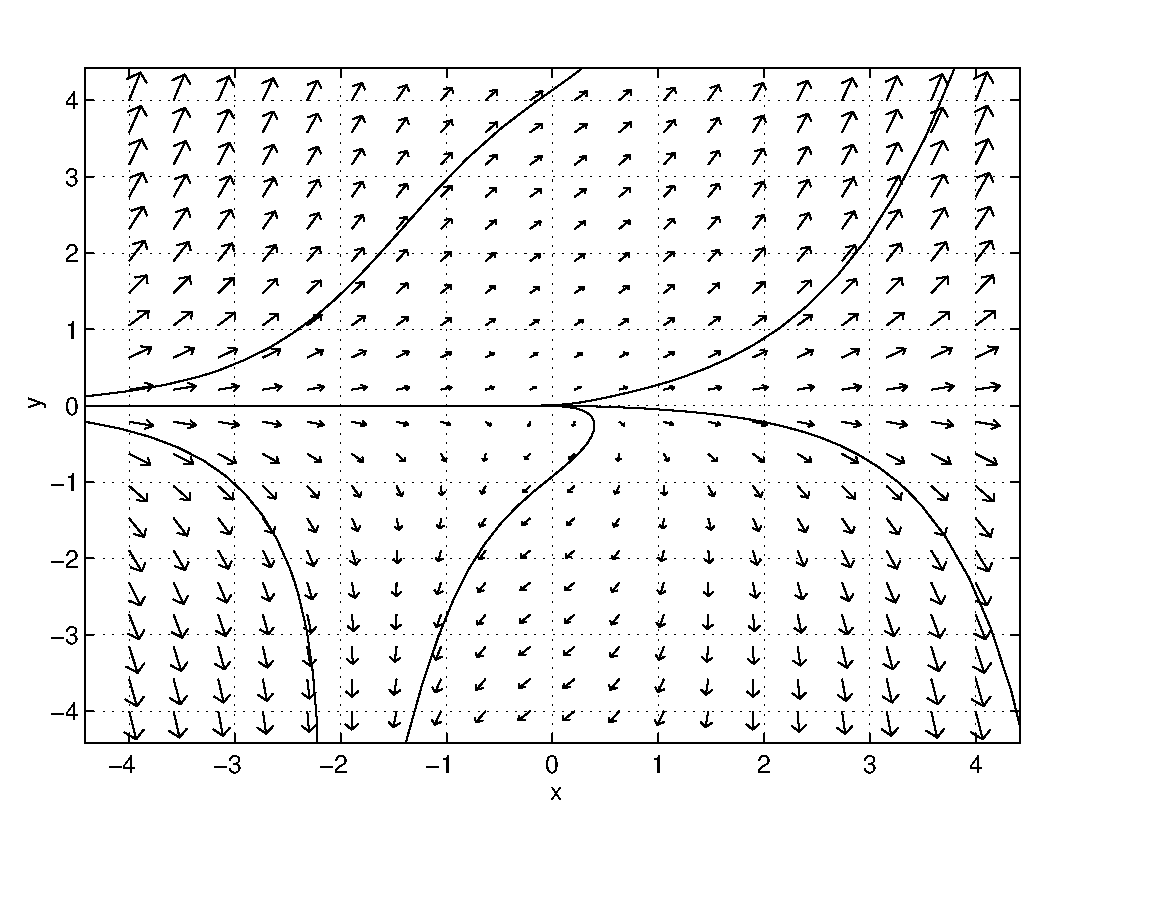
\psfig{file=exfigure/sourcea.eps,width=2.75in}
                       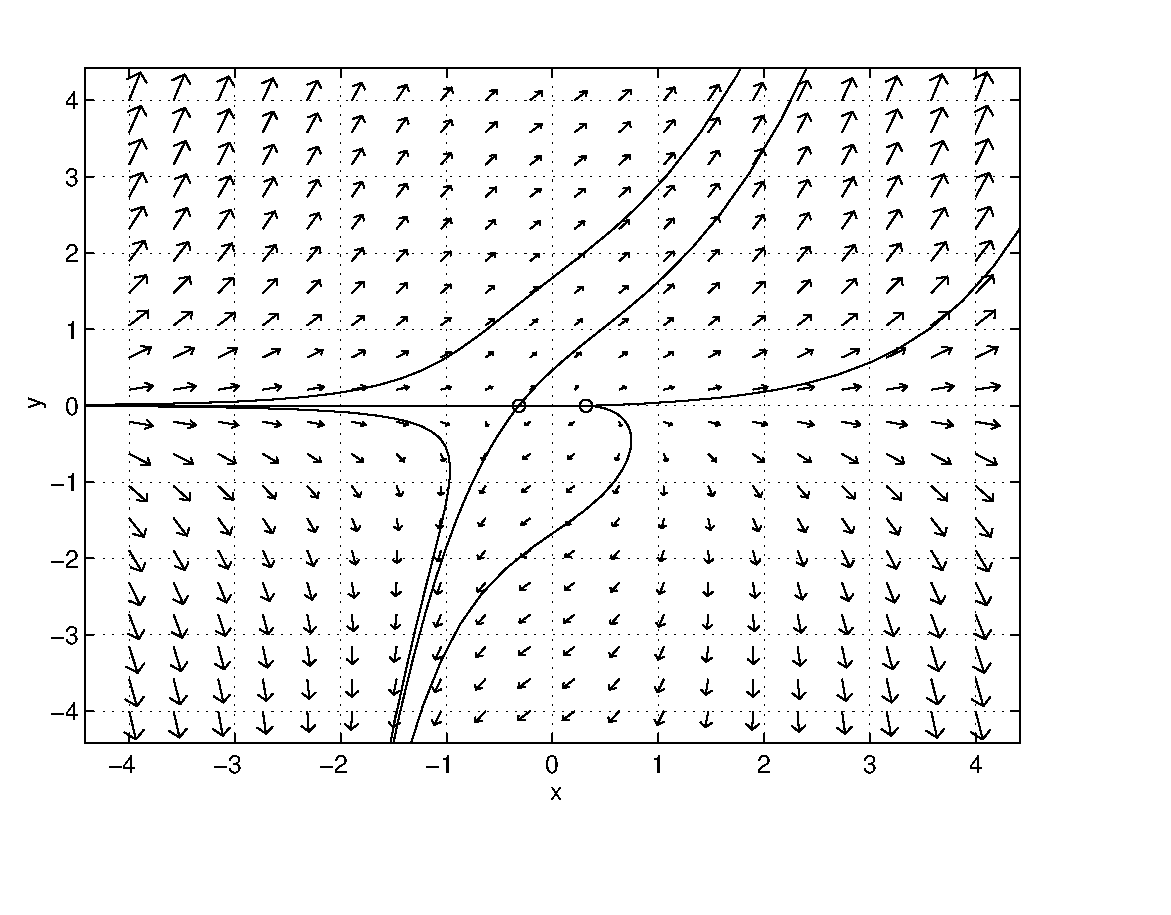
\psfig{file=exfigure/sourceb.eps,width=2.75in}}
                \exercaptwo{e:source}
\end{figure}

\exer{e:uHopf}
The system is shown in Figure~\ref{e:uHopf}a with $\rho = -1$, and in
Figure~\ref{e:uHopf}b with $\rho = 1$.  In this system, a limit cycle
exists before the bifurcation point, whereas, in \Ref{E:Hopfbif}, the
limit cycle exists after the bifurcation point and vanishes at
$\rho = 0$.  Also, in this system, the limit cycle is unstable, while
the limit cycle of \Ref{E:Hopfbif} is stable.

\begin{figure}[htb]
                       \centerline{%
                       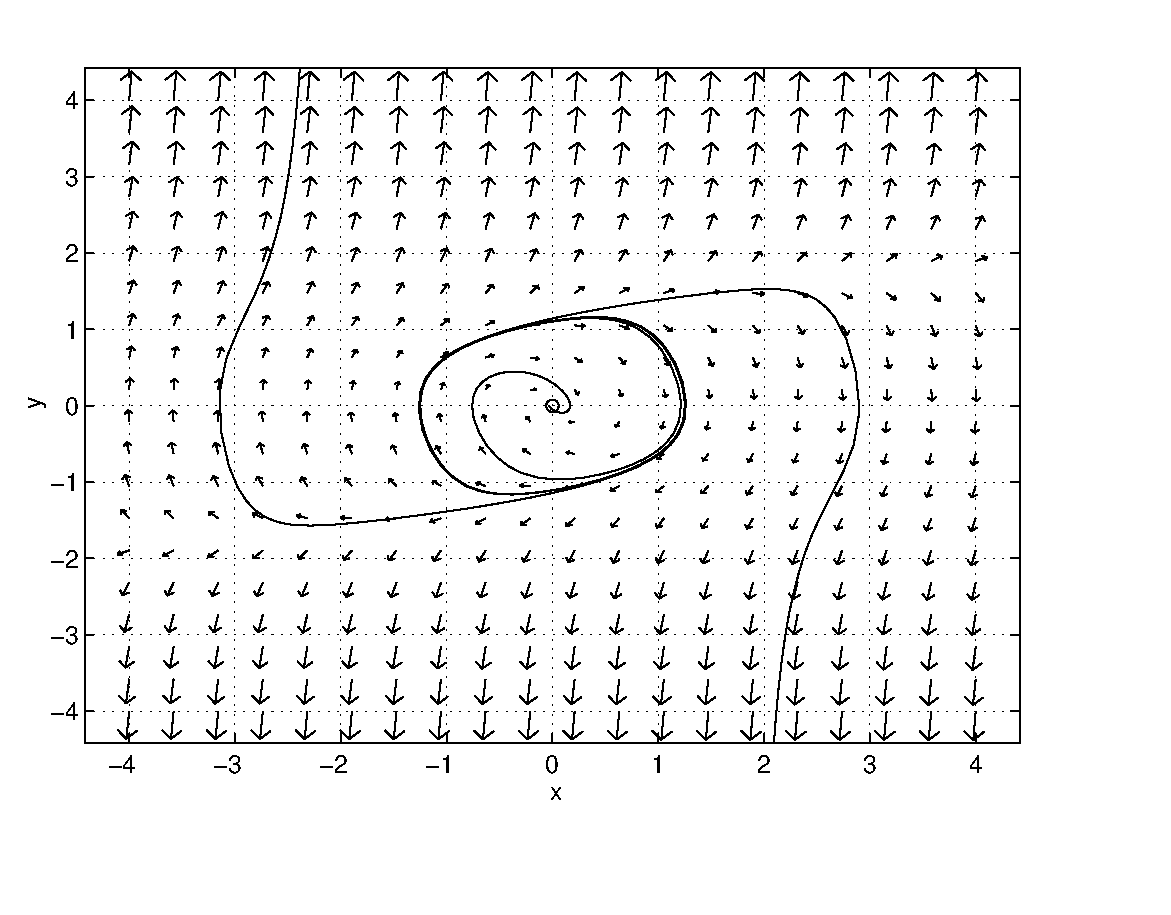
\psfig{file=exfigure/uHopfa.eps,width=2.75in}
                       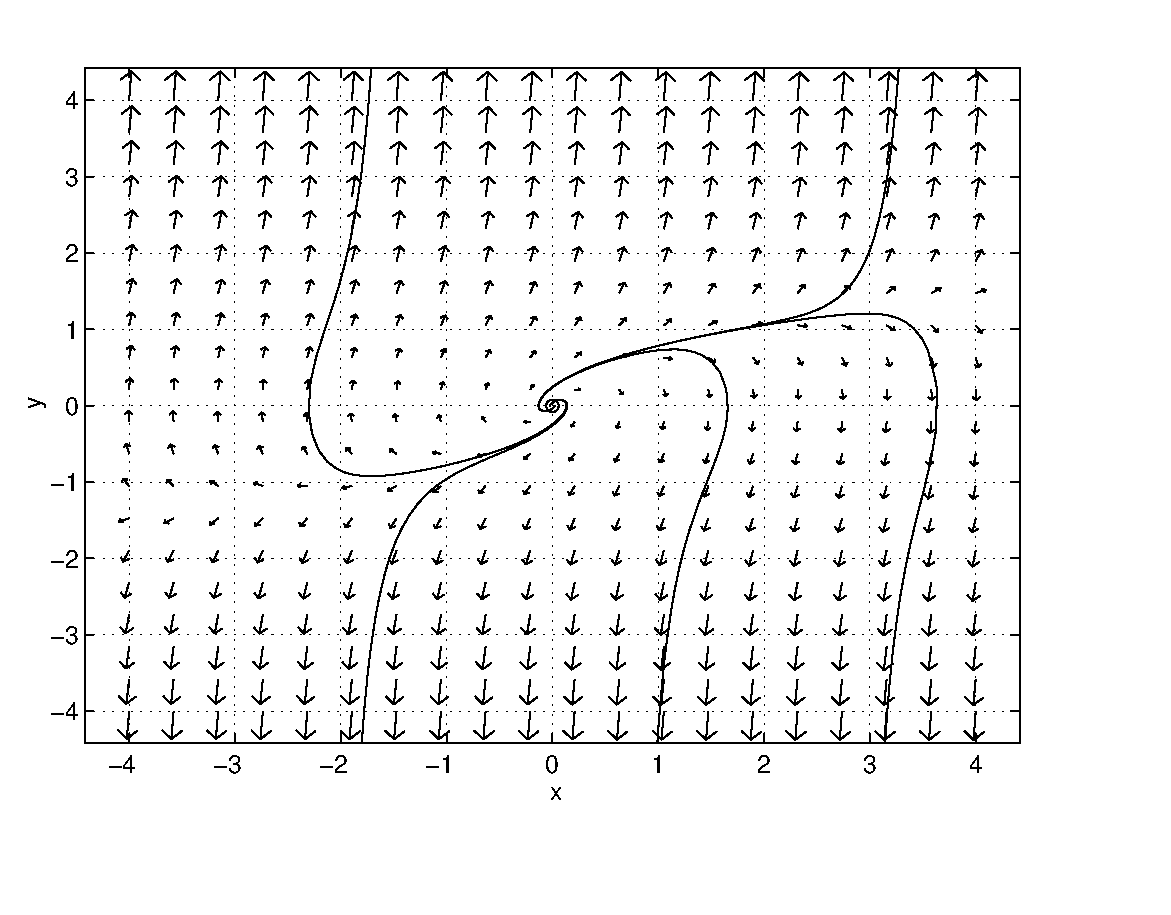
\psfig{file=exfigure/uHopfb.eps,width=2.75in}}
                \exercaptwo{e:uHopf}
\end{figure}

\exer{c9.7.4}
\ans (c) The system has a spiral sink when $\rho<-1$; (d) limit cycles exist 
when $\rho>-1$; a second Hopf bifurcation occurs near $\rho=-0.4$.


\soln  The differential equation \Ref{E:hbifex} is:
\[
\begin{array}{rcl}
\dot{x} & = & -1 + \rho + 5x + 2.5y + x^2 - x^3 \\
\dot{y} & = & -5 - x + 4y - y^2.  \end{array}
\]
(a) Substitute $x=-1$, $y=2$, and $\rho=-1$ into these equations to 
verify that $X_0=(-1,2)$ is an equilibrium when $\rho=-1$.

(b) The Jacobian matrix of this system at $X_0$ is:
\[
J = (dF)_{X_0} = \left.\cmattwo{5 + 2x-3x^2}{2.5}{-1}{4-2y}\right|_{(-1,2)}
= \mattwo{0}{2.5}{-1}{0}.
\]
Since $\trace(J)=0$ and $\det(J)=2.5>0$, $X_0$ is a center.

(c) Figure~\ref{c9.7.4}a shows the phase portrait for $\rho=-1.1$ and 
Figure~\ref{c9.7.4}b for $\rho=-0.9$.  From these figures we can conclude 
that the system has a spiral sink when $\rho<-1$.

(d) Limit cycles exist when $\rho>-1$.

(e)  As $\rho$ increases from $-1$, {\sf pplane5} shows that the limit 
cycle shrinks and disappears before $\rho=-0.1$. Numerical exploration
suggests that there is a Hopf bifurcation when $\rho\approx -0.4$.

\begin{figure}[htb]
                       \centerline{%
                       \psfig{file=exfigure/9-7-4a.eps,width=2.75in}
                       \psfig{file=exfigure/9-7-4b.eps,width=2.75in}}
                \exercaptwo{c9.7.4}
\end{figure}


\exer{c9.7.5} \soln
(a) The differential equation \Ref{e:homo} is:
\[
\begin{array}{rcl}
\dot{x} & = &  y \\
\dot{y} & = &  -\rho + y + x^2 + xy
\end{array}
\]
Solve the system for $\dot{x} = 0 = \dot{y}$ to find that the equilibria
occur at $y = 0$ and $x^2 = \rho$, which is $(\pm\sqrt{\rho},0)$
for $\rho > 0$.

(b)  The Jacobian matrix of these equations is:
\[
J_{(x,y)} = \cmattwo{0}{1}{2x+y}{1+x}.
\]
At the equilibria $(\pm\sqrt{\rho},0)$ the Jacobians are
\[
J_{(\sqrt{\rho},0)}= \cmattwo{0}{1}{2\sqrt{\rho}}{1+\sqrt{\rho}} 
\AND
J_{(-\sqrt{\rho},0)}= \cmattwo{0}{1}{-2\sqrt{\rho}}{1-\sqrt{\rho}}
\]
The first Jacobian has determinant equal to $-2\sqrt{\rho}<0$; so the
first equilibrium is always a saddle.  The second Jacobian has determinant
equal to $2\sqrt{\rho}>0$ and trace equal to $1-\sqrt{\rho}$.  Since the
trace is negative when $\rho>1$, the second equilibrium is a sink.  The
discriminant of the second Jacobian is 
\[
(1-\sqrt{\rho})^2-8\sqrt{\rho}=1-10\sqrt{\rho}+\rho.
\]
The second equilibrium is a spiral when the discriminant is negative, which
it is when $1<\rho<97$.

(c)  Figures~\ref{c9.7.5}a and \ref{c9.7.5}b show that a homoclinic 
bifurcation has occurred between parameter values $\rho=1.7$ (a) and 
$\rho=1.8$ (b) with its characteristic loss of a limit cycle. 

\begin{figure}[htb]
                       \centerline{%
                       \psfig{file=exfigure/9-7-5a.eps,width=2.75in}
                       \psfig{file=exfigure/9-7-5b.eps,width=2.75in}}
                \exercaptwo{c9.7.5}
\end{figure}

\exer{c9.4.3a}
The Jacobian of \Ref{E:duff} at the origin is
\[
J_{(0,0,\mu)} = \cmattwo{-\mu}{1}{-1}{-\mu}.
\]
Let $\mu = 0$.  Then $\trace(J_{(0,0,0)}) = -2\mu = 0$ and
$\det(J_{(0,0,0)}) = \mu^2 + 1 = 1 > 0$.  The trace moves through $0$ with
nonzero speed since
\[
\frac{d}{d\mu}\trace(J_{(0,0,0)}) = \frac{d}{d\mu}(-2\mu) = -2 \neq 0.
\]
Thus, \Ref{E:duff} undergoes a Hopf bifurcation near the origin when
$\mu = 0$.  Figure~\ref{c9.4.3a} shows the system with $\mu = 0.05$.  At
this point, the origin is a source.  Figure~\ref{c9.4.3b} shows the
system with $\mu = -0.05$.  At this point, the origin is a sink, and there
is a periodic solution.

\exer{c9.4.3b}
There is a homoclinic bifurcation at $\mu \approx -0.1$.  To show this,
compare Figure~\ref{c9.4.3b} with Figure~\ref{c9.4.3c}, which shows the
system with $\mu = -0.15$.  At $\mu = -0.15$, there is no longer a periodic
solution around the origin.  The bifurcation point occurs when the stable
and unstable orbits of the saddle point in the first quadrant coincide.

\exer{c9.4.3c}
When $\mu > 0$, all solutions with initial conditions between the
stable orbits of the saddle point stay within the square $-2 \leq
x,y \leq 2$ in forward time, and no solutions stay within this region
for all time.

\para When $-0.1 < \mu < 0$, all solutions with initial
conditions between the stable orbits of the saddle point stay within the
region in forward time.  Solutions with initial conditions inside the
periodic orbit stay within the region in backward time also.

\para When $\mu < -0.1$, only solutions with initial conditions along the
stable orbits of the saddle point stay within the region in forward time,
and no solutions stay within the region for all time.

\begin{figure}[htb]
                       \centerline{%
                       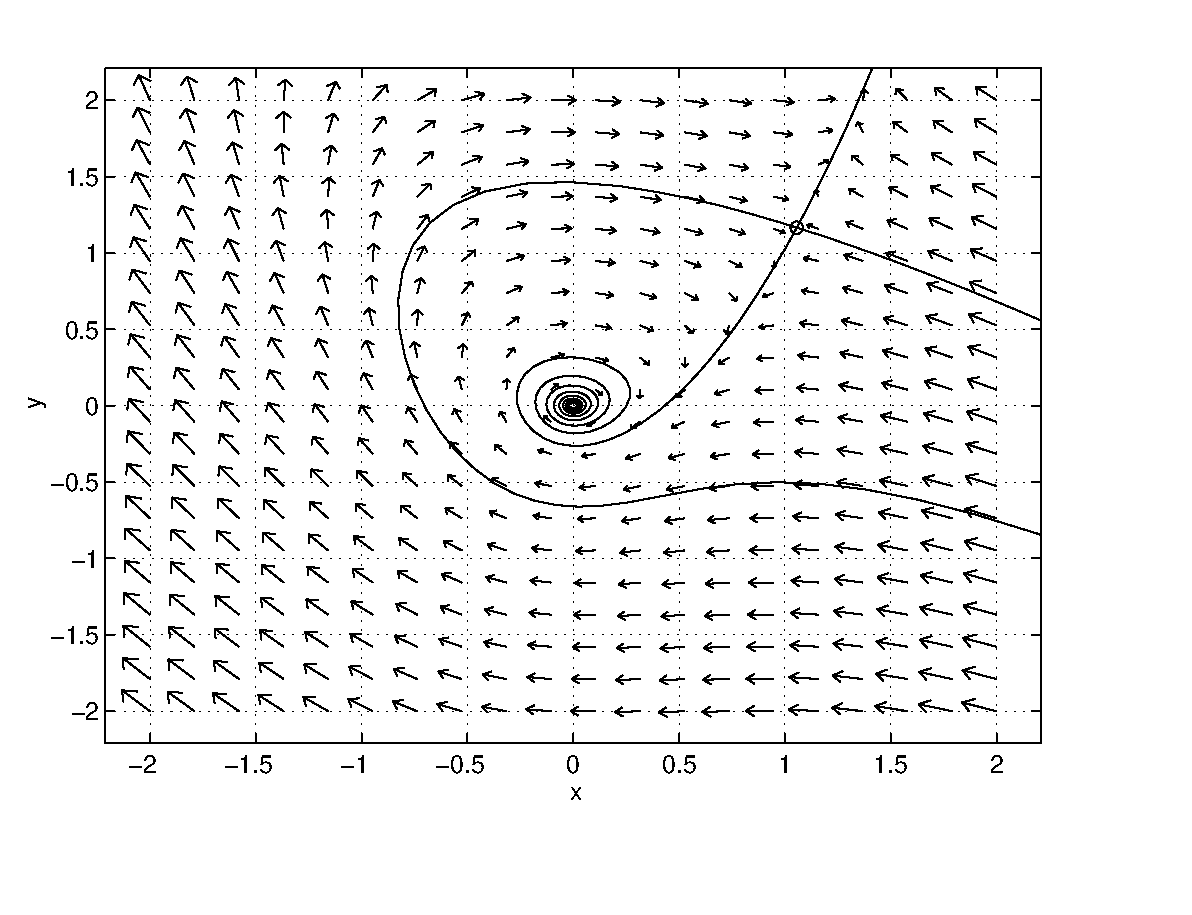
\psfig{file=exfigure/9-4-3a.eps,width=1.8in}
                       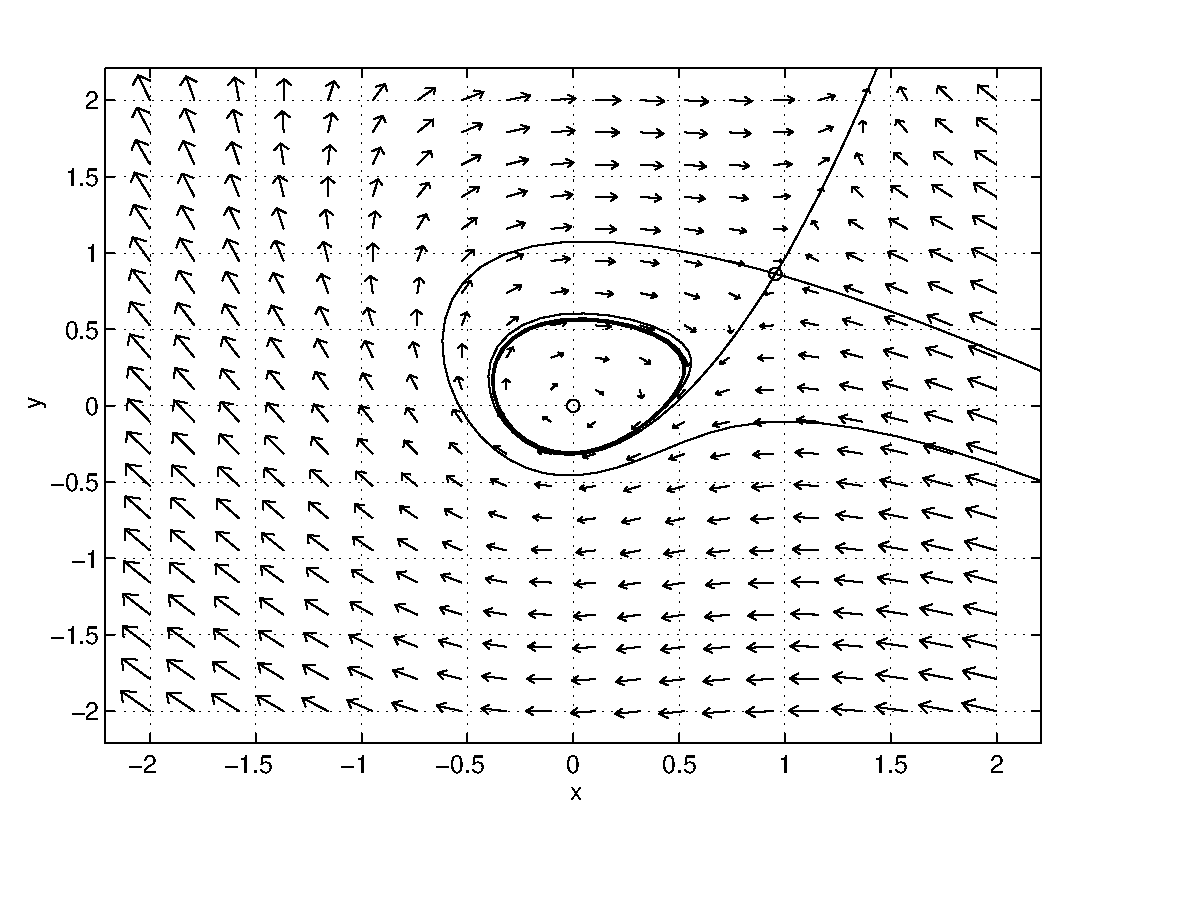
\psfig{file=exfigure/9-4-3b.eps,width=1.8in}
                       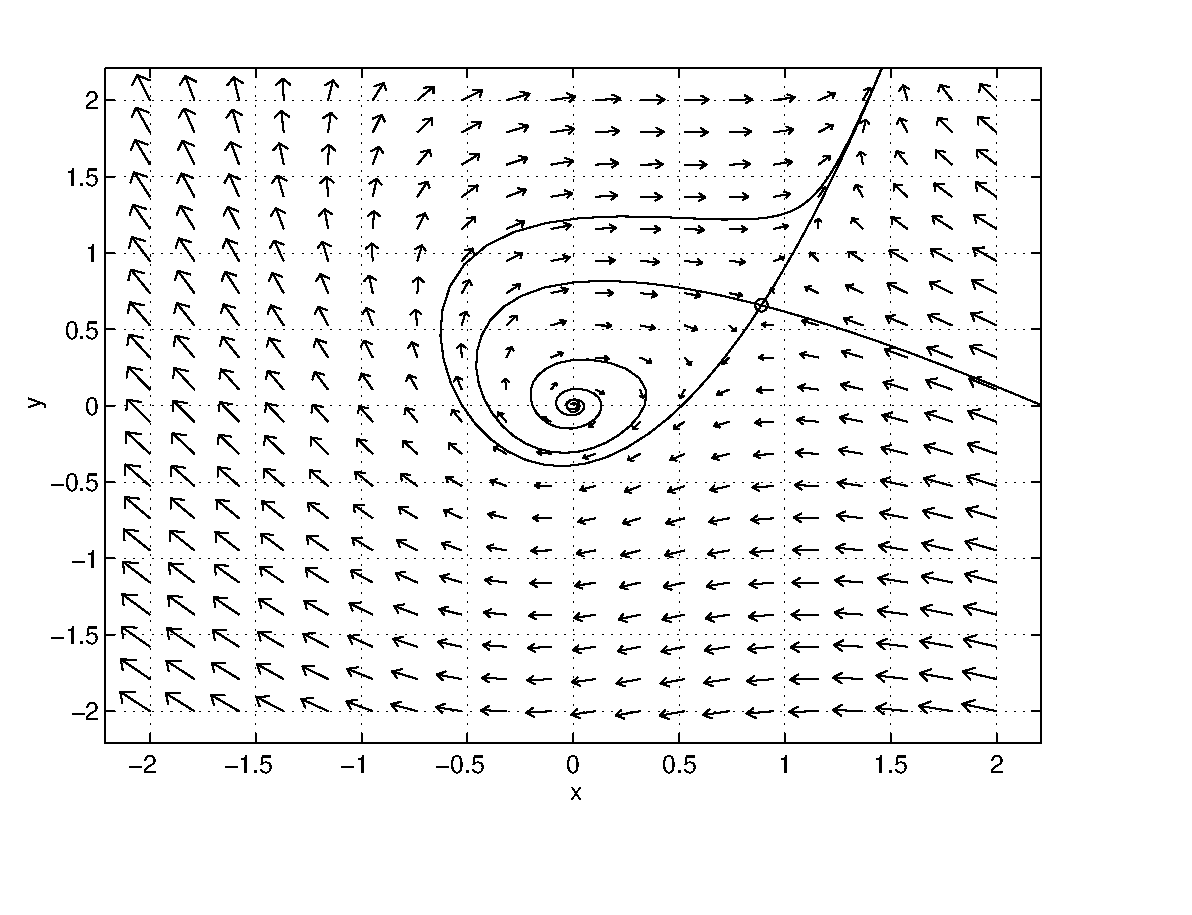
\psfig{file=exfigure/9-4-3c.eps,width=1.8in}}
		\centerline{$\mu > 0$\hspace{1.2in}$-0.1 < \mu < 0$
\hspace{1.2in}$\mu < -0.1$}
		\centerline{Figure~\ref{c9.4.3a}\hspace{1.2in}
Figure~\ref{c9.4.3b}\hspace{1.2in}Figure~\ref{c9.4.3c}}
\end{figure}

\exer{c9.4.4}
\ans The system has small amplitude periodic solutions when $\rho > 0$.

\soln Load the system into \Matlab, and graph the
system for small positive and negative values of $\rho$.



\newpage
\subsection*{Section~\protect{\ref{S:CSTR}} The Continuous Flow Stirred Tank
Reactor}
\rhead{S:CSTR}{THE CONTINUOUS FLOW STIRRED TANK REACTOR}

\exer{E:CSTR5}
The system is shown in Figure~\ref{E:CSTR5}a with $\rho = 0.5$, and in
Figure~\ref{E:CSTR5}b with $\rho = 0.505$.  Note that, due to rounding
error, {\tt pplane5} may calculate the middle temperature equilibrium of
the first system as a saddle rather than a saddle node.  

\begin{figure}[htb]
                       \centerline{%
                       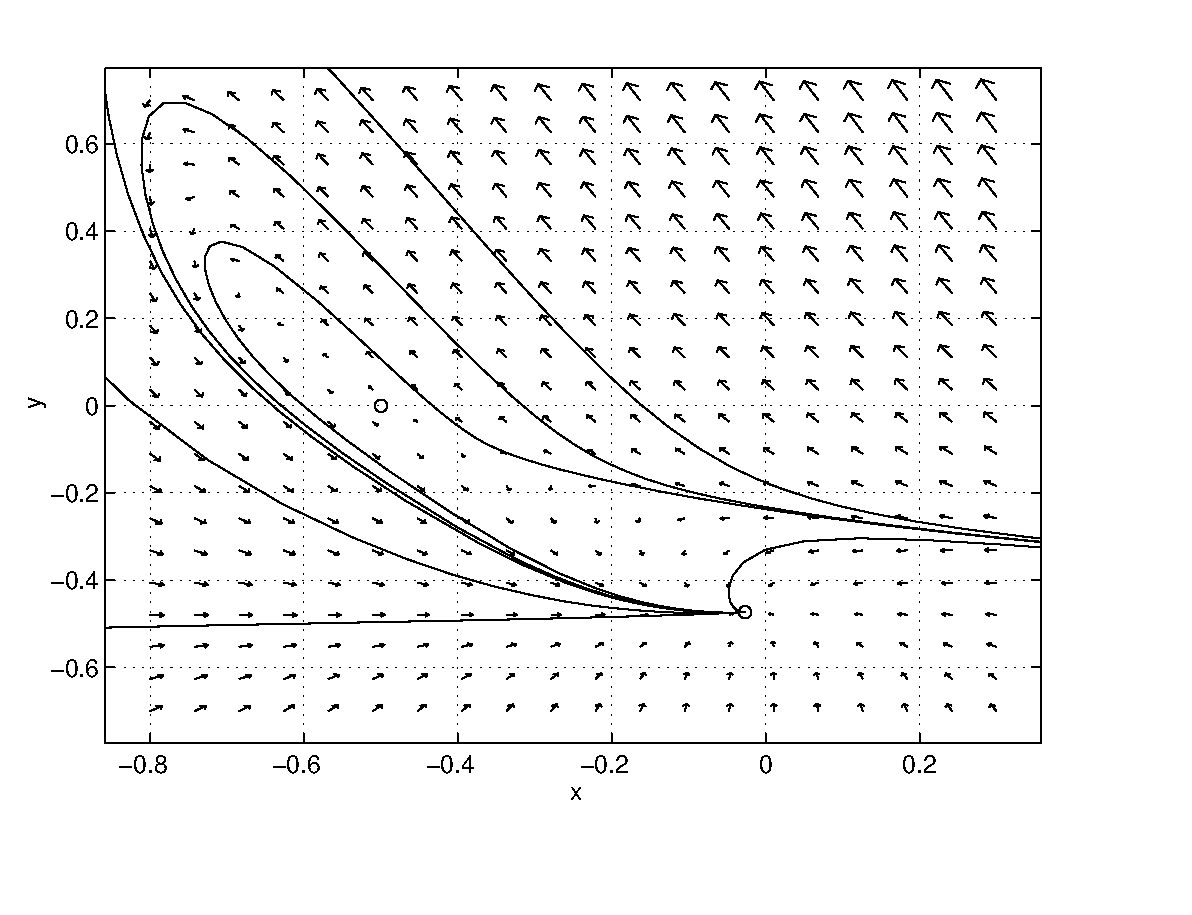
\psfig{file=exfigure/CSTR5a.eps,width=2.75in}
                       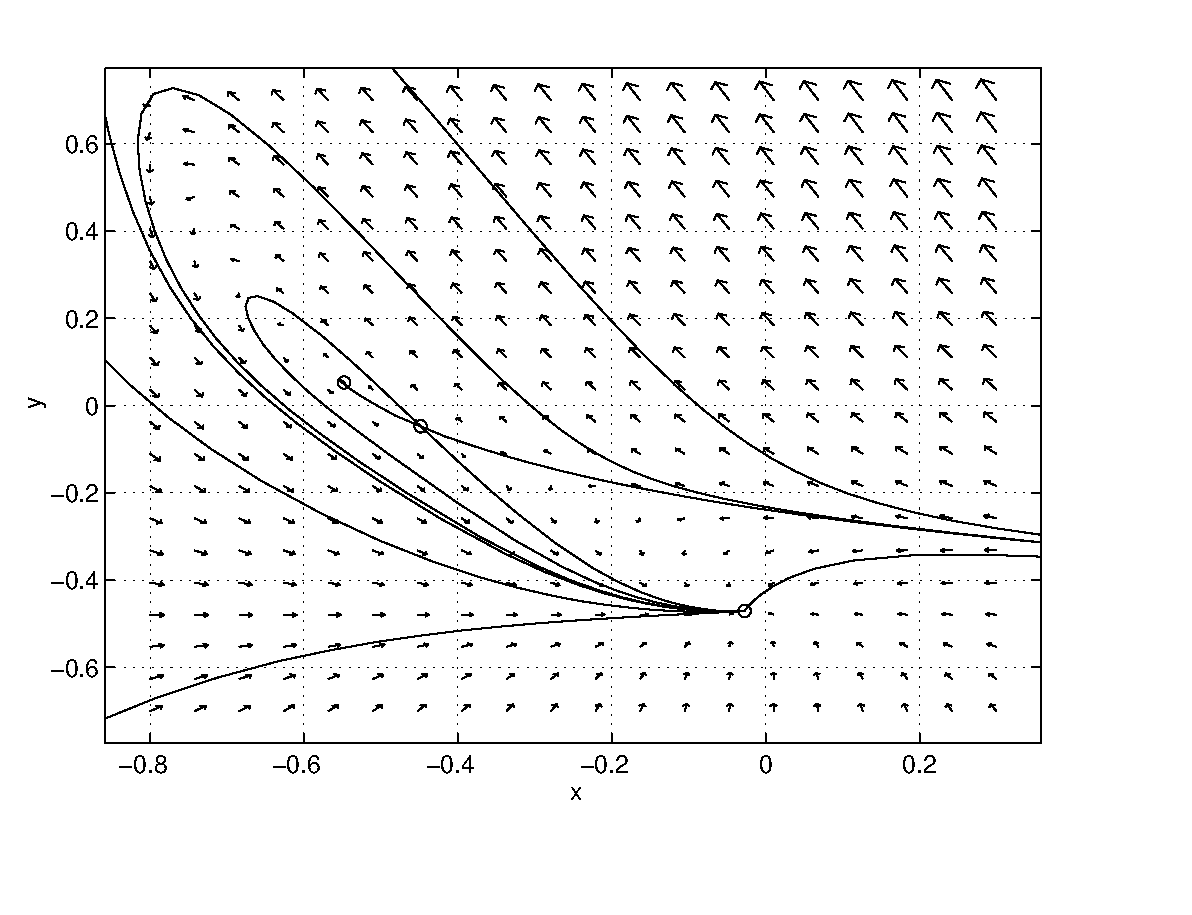
\psfig{file=exfigure/CSTR5b.eps,width=2.75in}}
                \exercaptwo{E:CSTR5}
\end{figure}

\exer{c9.2.2}
With these parameter values and $0.46 \leq \rho \leq 0.51$, the system
has one equilibrium near $(-0.4,-0.1)$.  There are two values of $\rho$
at which Hopf bifurcation occurs: $\rho \approx 0.46735$ and
$\rho = 0.5$.  At these values of $\rho$, there is a periodic solution
around the equilibrium.  For $0.46 \leq \rho < 0.46735$ or $0.5 < \rho
\leq 0.51$, the equilibrium is a spiral sink.  Between the two
bifurcations, the equilibrium is a spiral source.  Figure~\ref{c9.2.2}a
shows the {\tt pplane5} graph of the system with $\rho = 4.6$. 
Figure~\ref{c9.2.2}b shows a graph of the system with $\rho = 0.49$,
between the two bifurcation points.  Figure~\ref{c9.2.2}c shows a graph
of the system with $\rho = 0.5$, at one of the Hopf bifurcation points.
The bifurcation diagram of the system is shown in Figure~\ref{c9.2.2}d.

\begin{figure}[htb]
                       \centerline{%
                       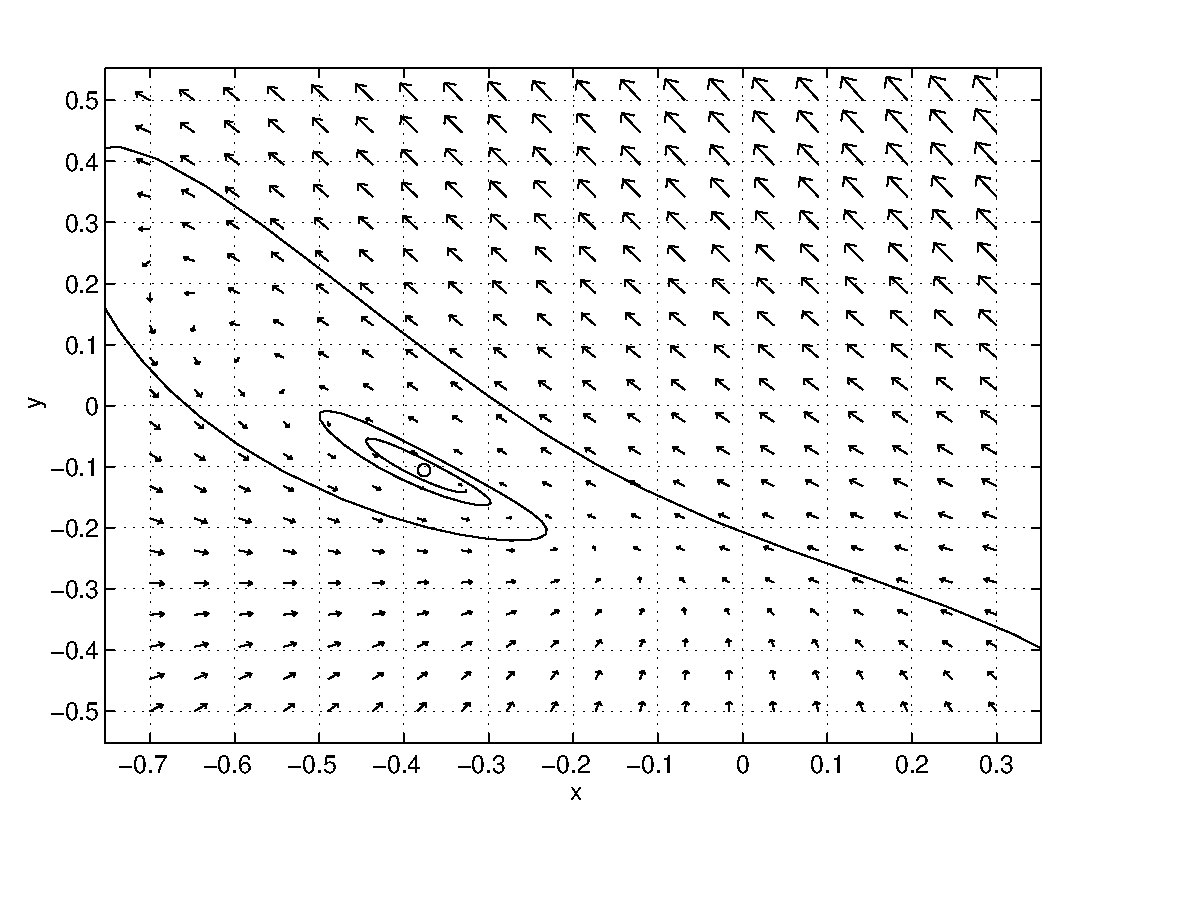
\psfig{file=exfigure/9-2-2a.eps,width=1.8in}
                       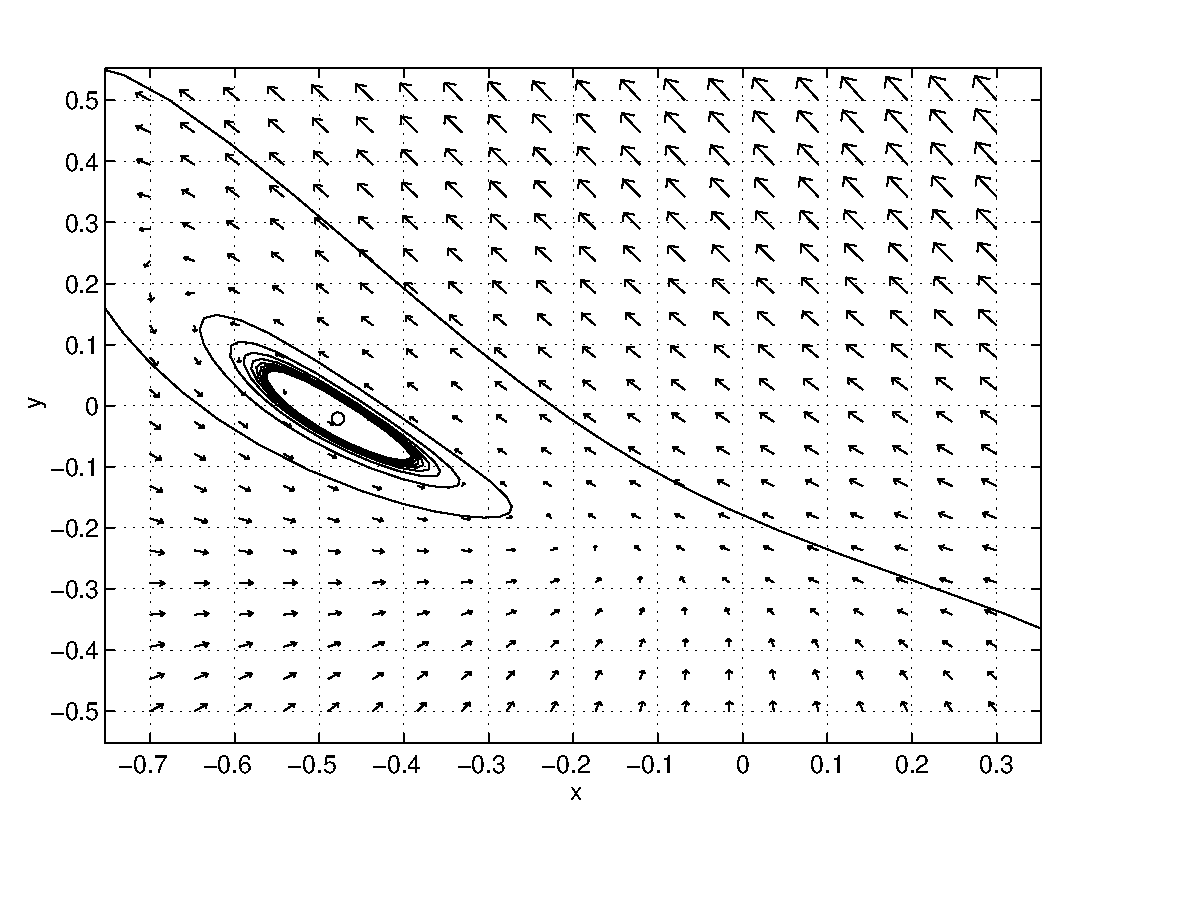
\psfig{file=exfigure/9-2-2b.eps,width=1.8in}
                       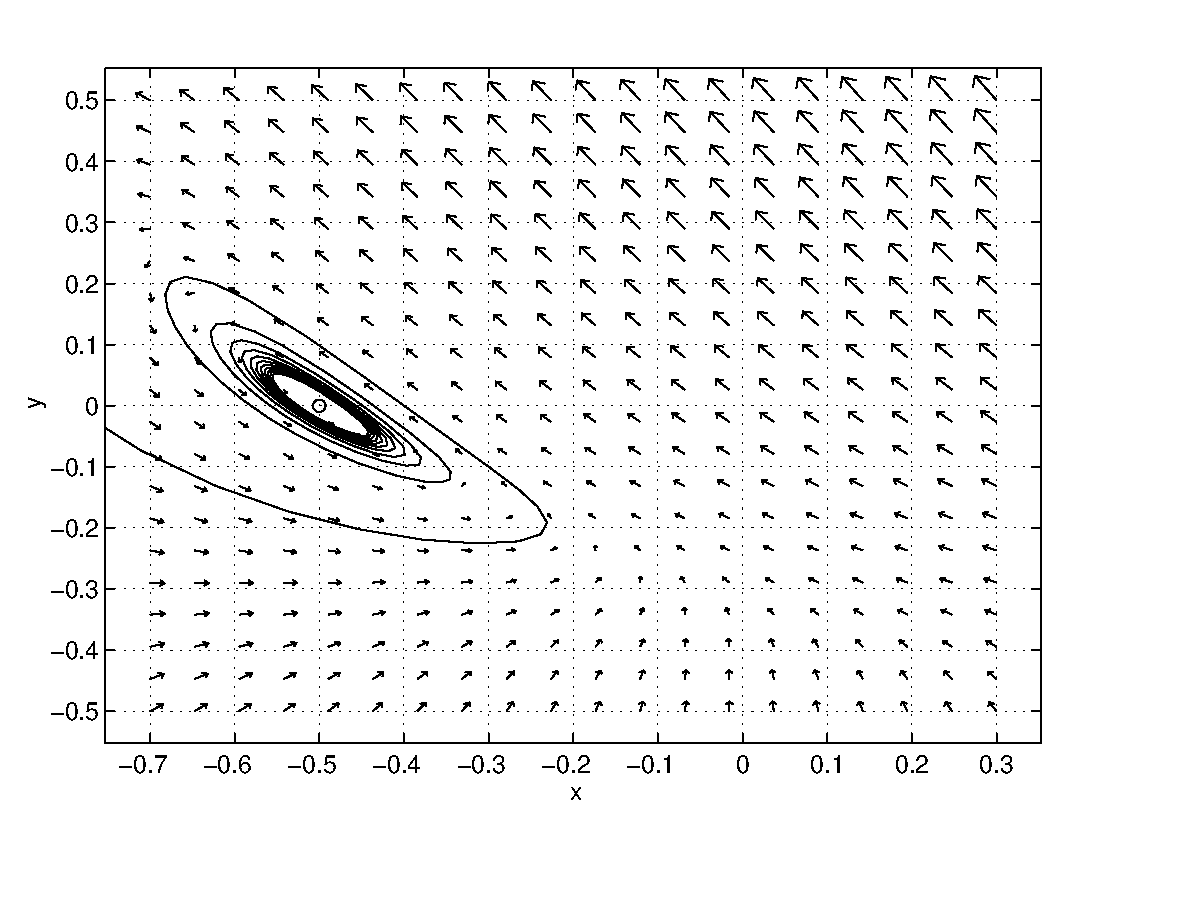
\psfig{file=exfigure/9-2-2c.eps,width=1.8in}}
                \exercapthree{c9.2.2}
\end{figure}

\begin{figure}[htb]
			\centerline{%
			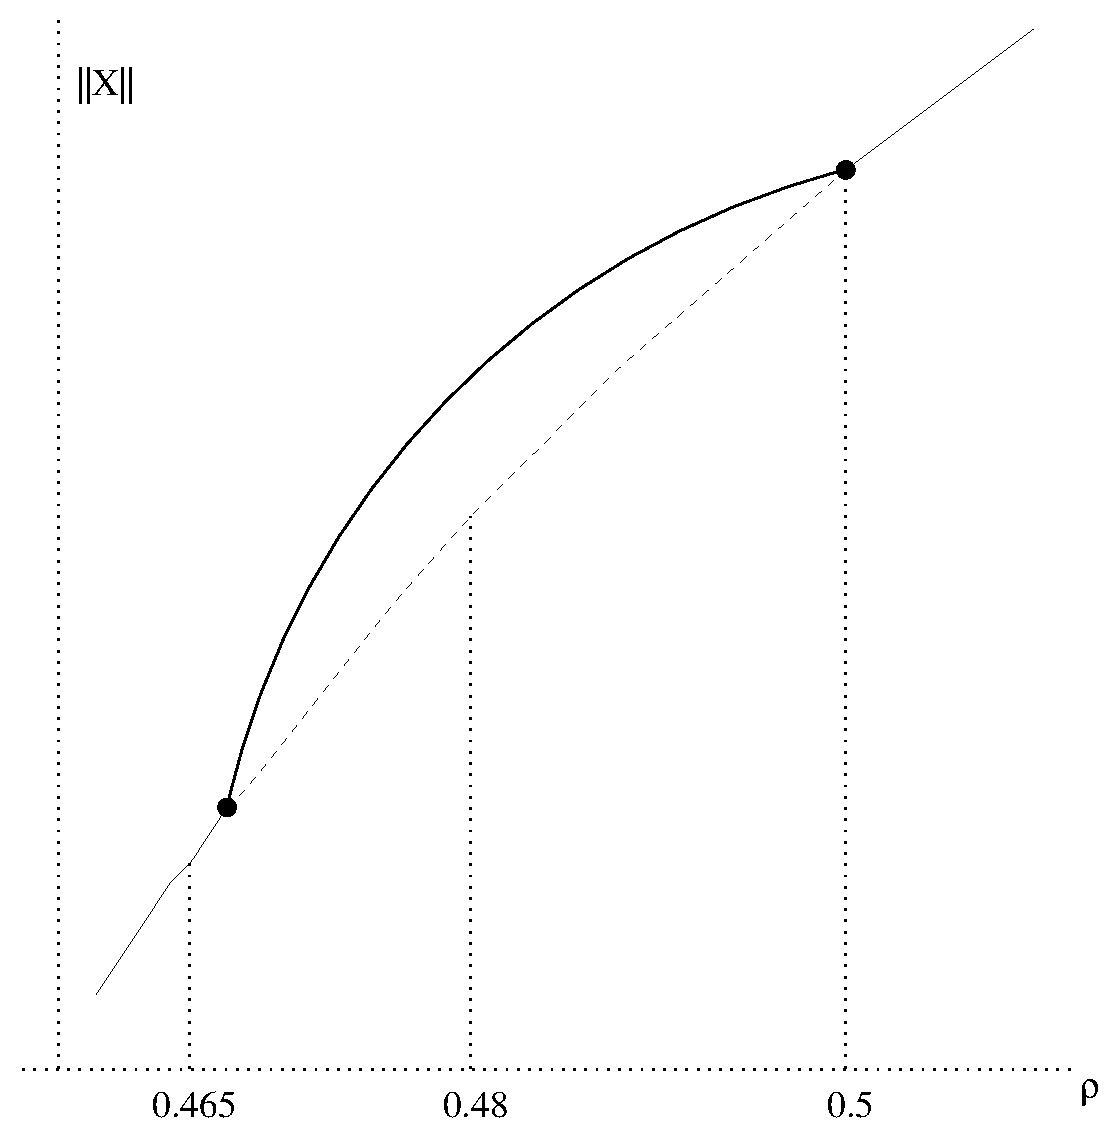
\psfig{file=exfigure/9-2-2d.eps,width=3.0in}}
		\centerline{Figure~\ref{c9.2.2}d}
\end{figure}



\subsection*{Section~\protect{\ref{S:GlobalBif}} The Remaining Global Bifurcations}
\rhead{S:GlobalBif}{THE REMAINING GLOBAL BIFURCATIONS}

\exer{c9.5.1}
The system has a saddle-node bifurcation of periodic solutions
at $\rho \approx 0.995$.  Figure~\ref{c9.5.1}a shows the system
with $\rho = 0.7$, at which point there are two limit cycles. 
Figure~\ref{c9.5.1}b shows the system with $\rho = 0.995$, near the point
of collision.  Figure~\ref{c9.5.1}c shows the system with $\rho = 1.1$, where
there are no periodic solutions.

\begin{figure}[htb]
                       \centerline{%
                       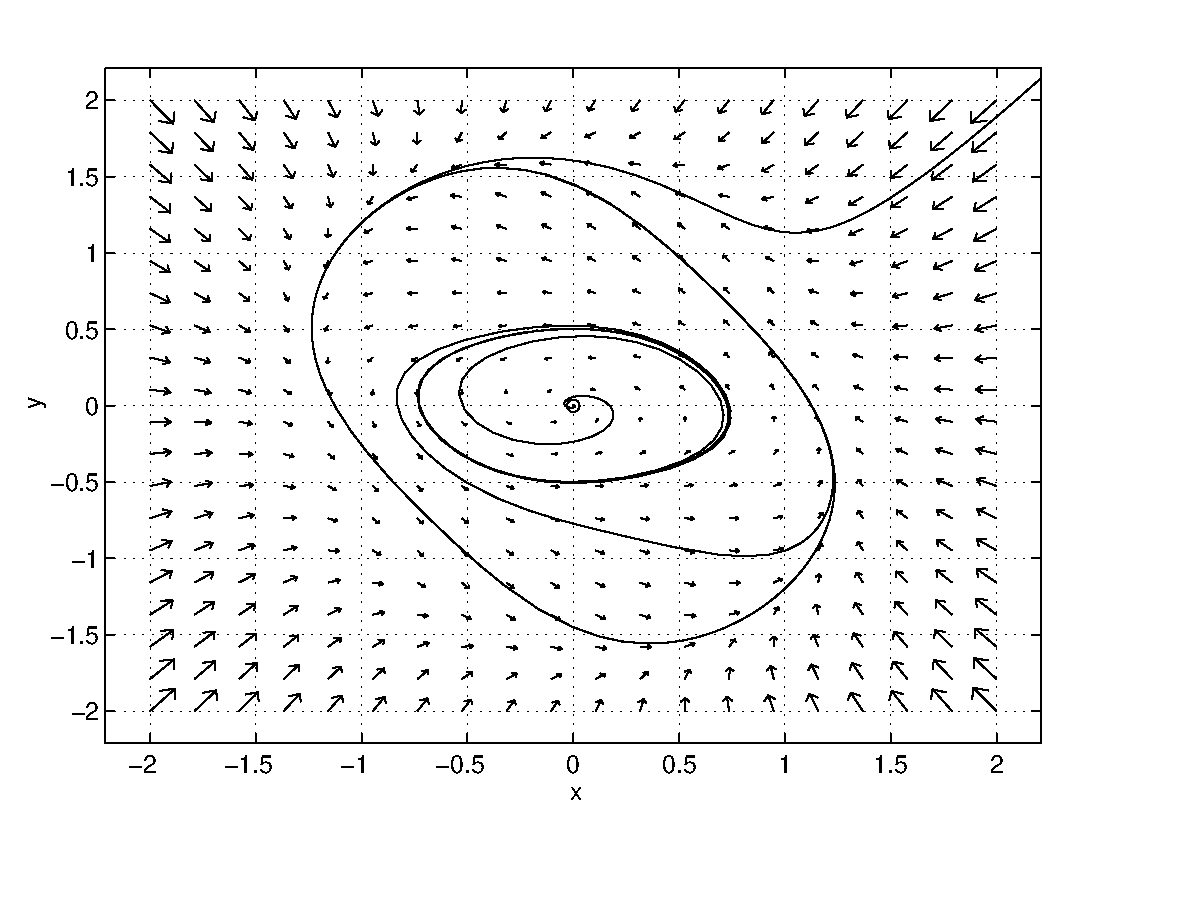
\psfig{file=exfigure/9-5-1a.eps,width=1.8in}
                       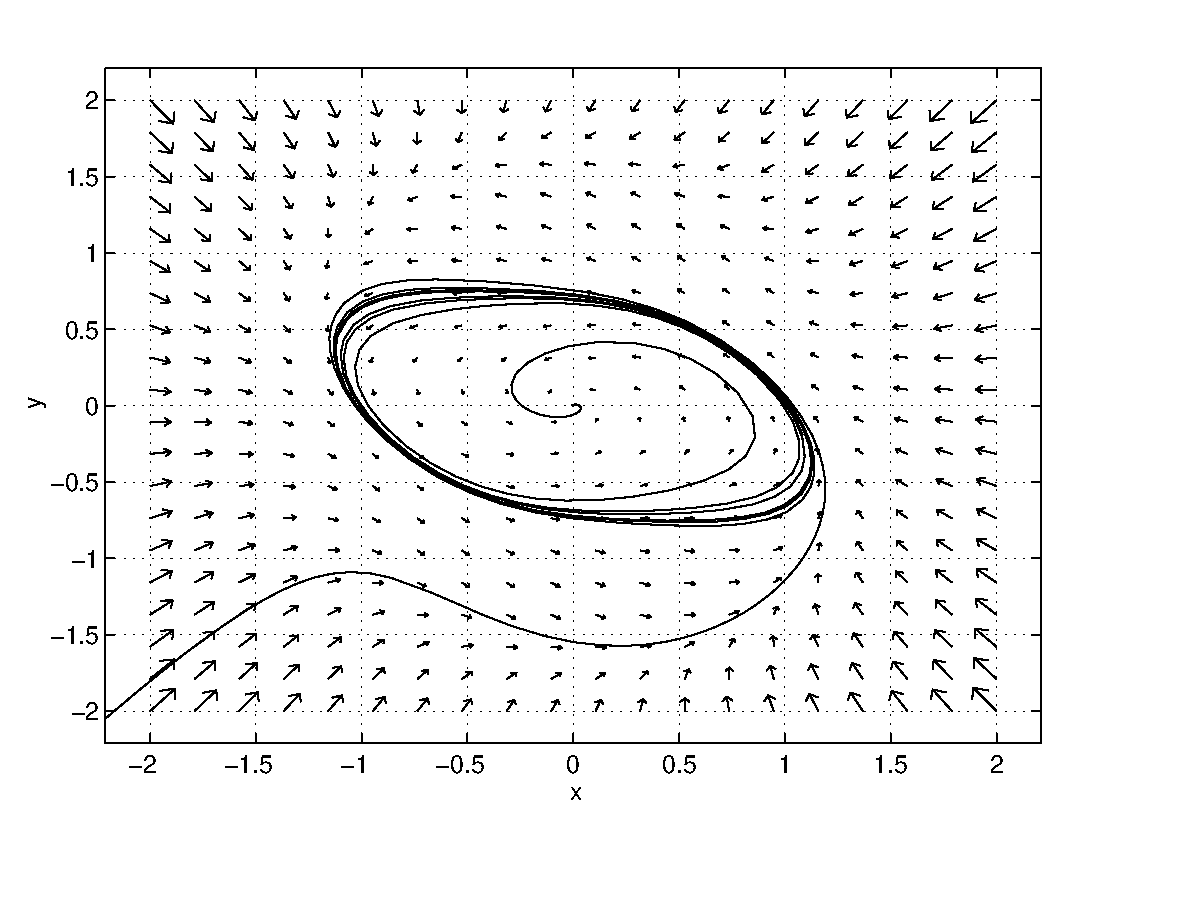
\psfig{file=exfigure/9-5-1b.eps,width=1.8in}
                       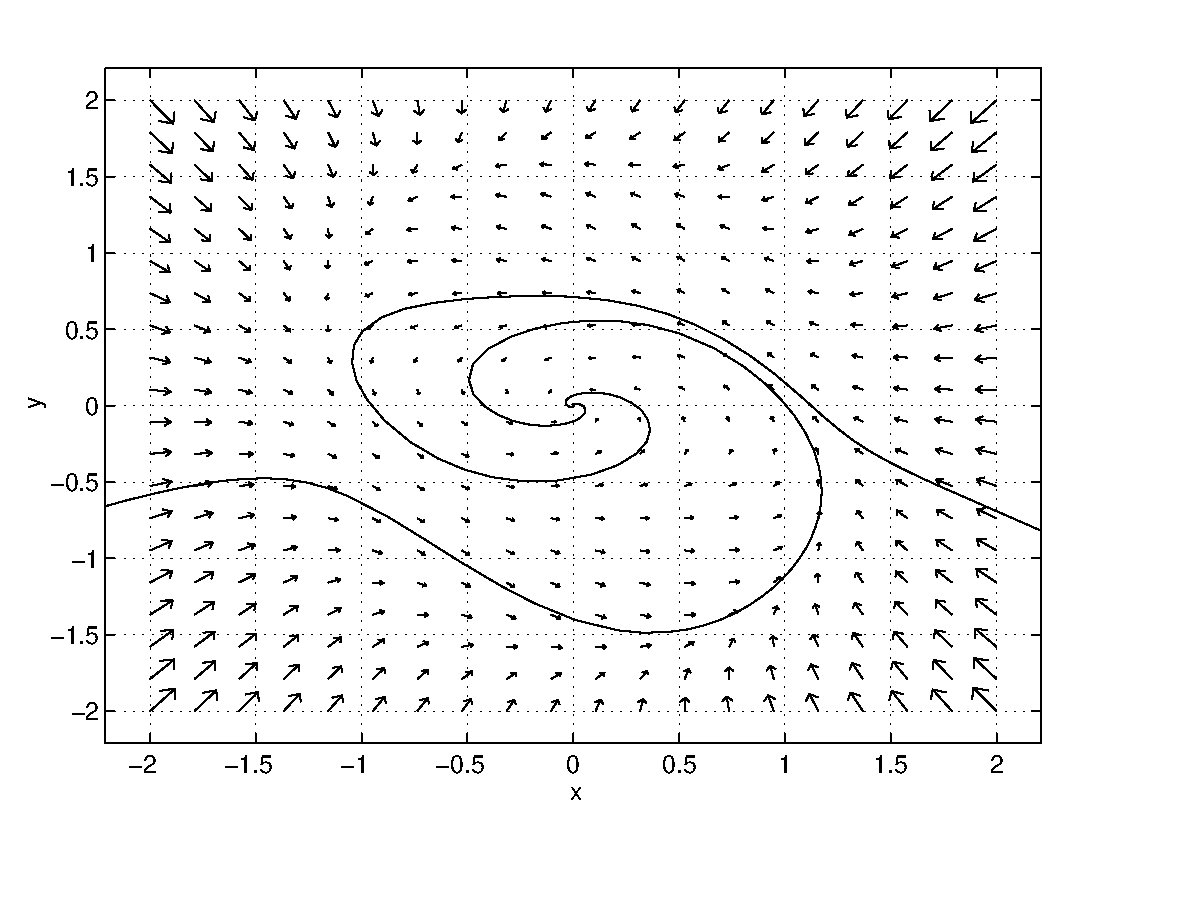
\psfig{file=exfigure/9-5-1c.eps,width=1.8in}}
		\centerline{$\rho = 0.7$\hspace{1.3in}$\rho = 0.995$
\hspace{1.3in}$\rho = 1.1$}
                \exercapthree{c9.5.1}
\end{figure}

\exer{c9.6.2a} Figure~\ref{c9.6.2a} shows the system with $\rho = -0.02$. 
At this point, there is a periodic solution around the origin.

\exer{c9.6.2b} Figure~\ref{c9.6.2b} shows the system with $\rho = -0.03$. 
At this point, there is no periodic solution.

\exer{c9.6.2c}
\ans By examination of {\tt pplane5} graphs of \Ref{E:homo2}, a homoclinic
bifurcation occurs near $\rho = -0.027$.

\soln 
Using {\tt pplane5}, graph the system as $\rho$ decreases from $-0.02$, and
note that the periodic solution disappears at when stable and unstable
orbits of the saddle point coincide.  This homoclinic bifurcation occurs
at $\rho \approx -0.027$.  Figure~\ref{c9.6.2c} shows the system with
$\rho = -0.027$.  Note that these figures are created by mapping the stable
and unstable trajectories of the saddle point.

\begin{figure}[htb]
                       \centerline{%
                       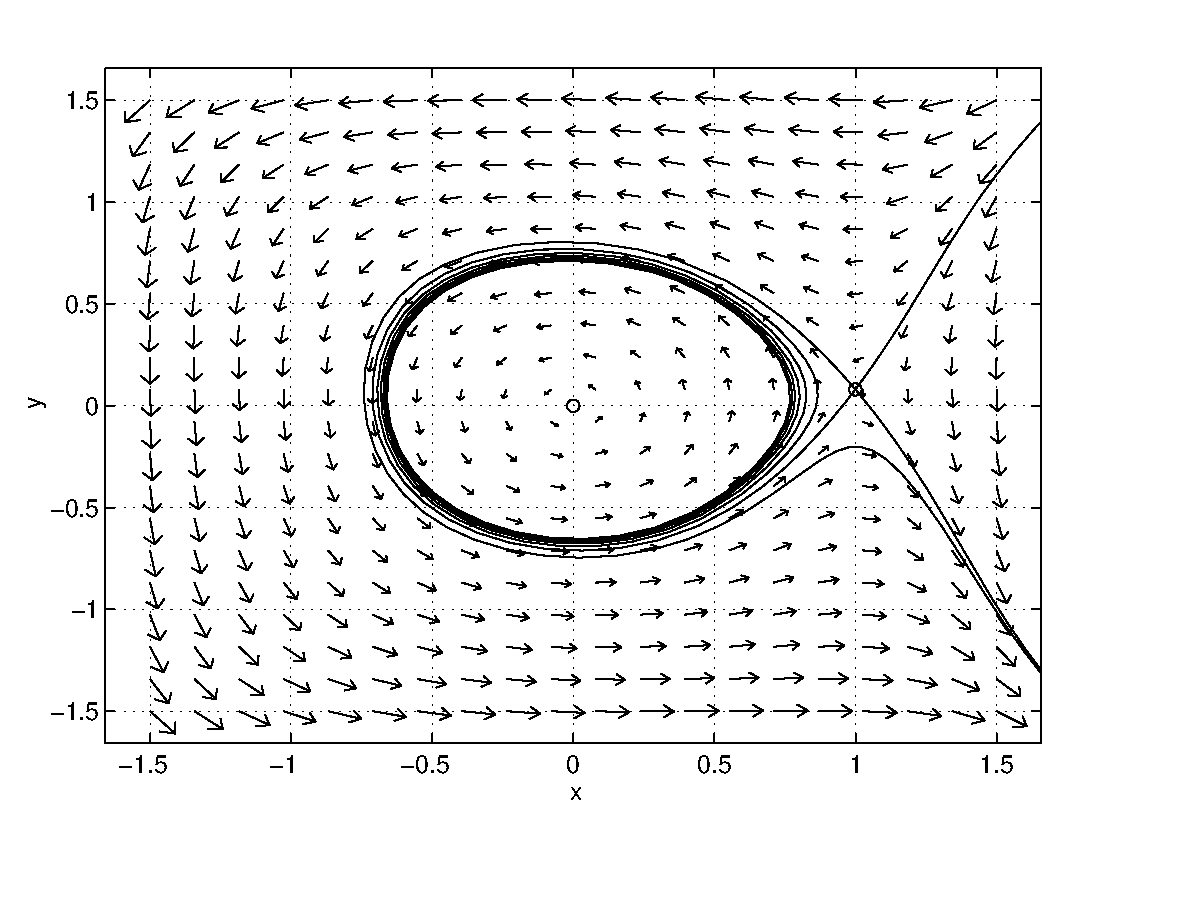
\psfig{file=exfigure/9-6-2a.eps,width=1.8in}
                       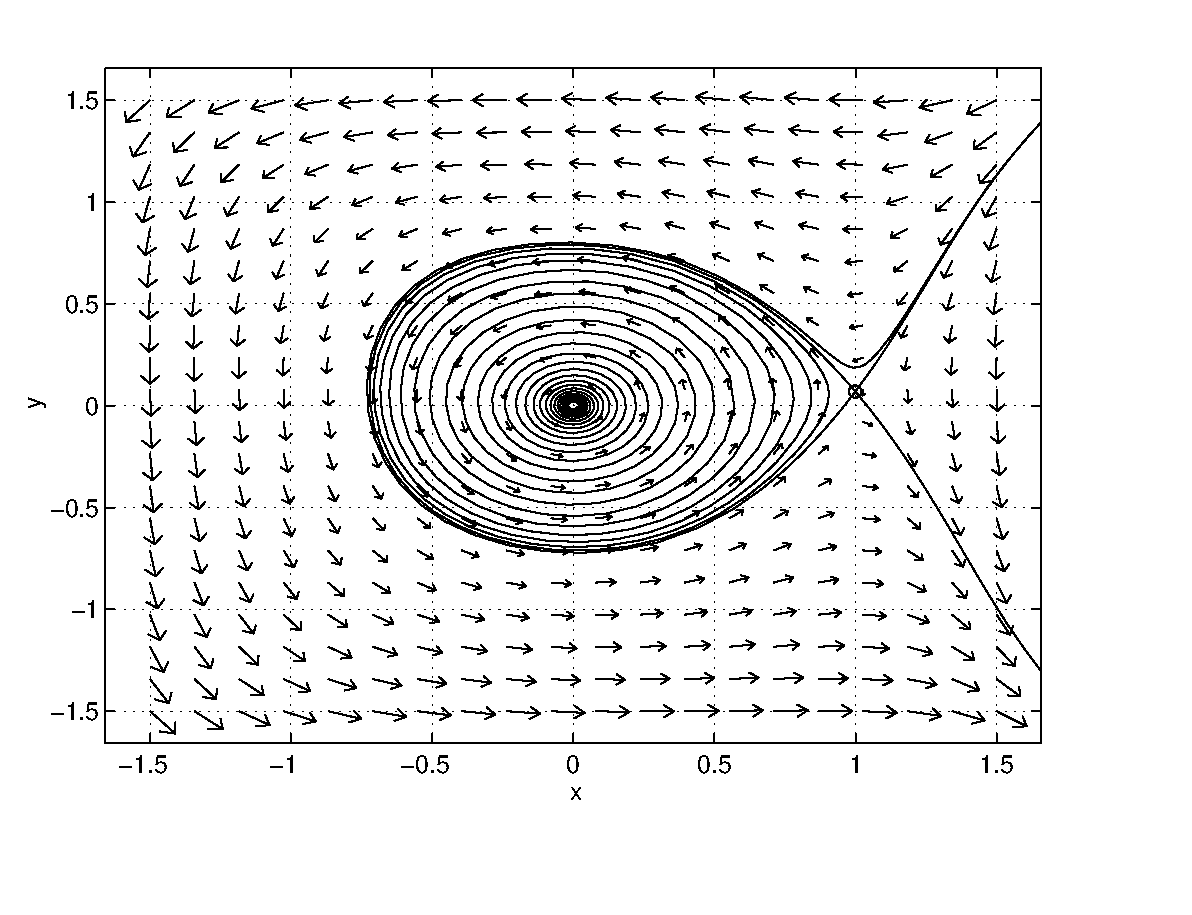
\psfig{file=exfigure/9-6-2b.eps,width=1.8in}
                       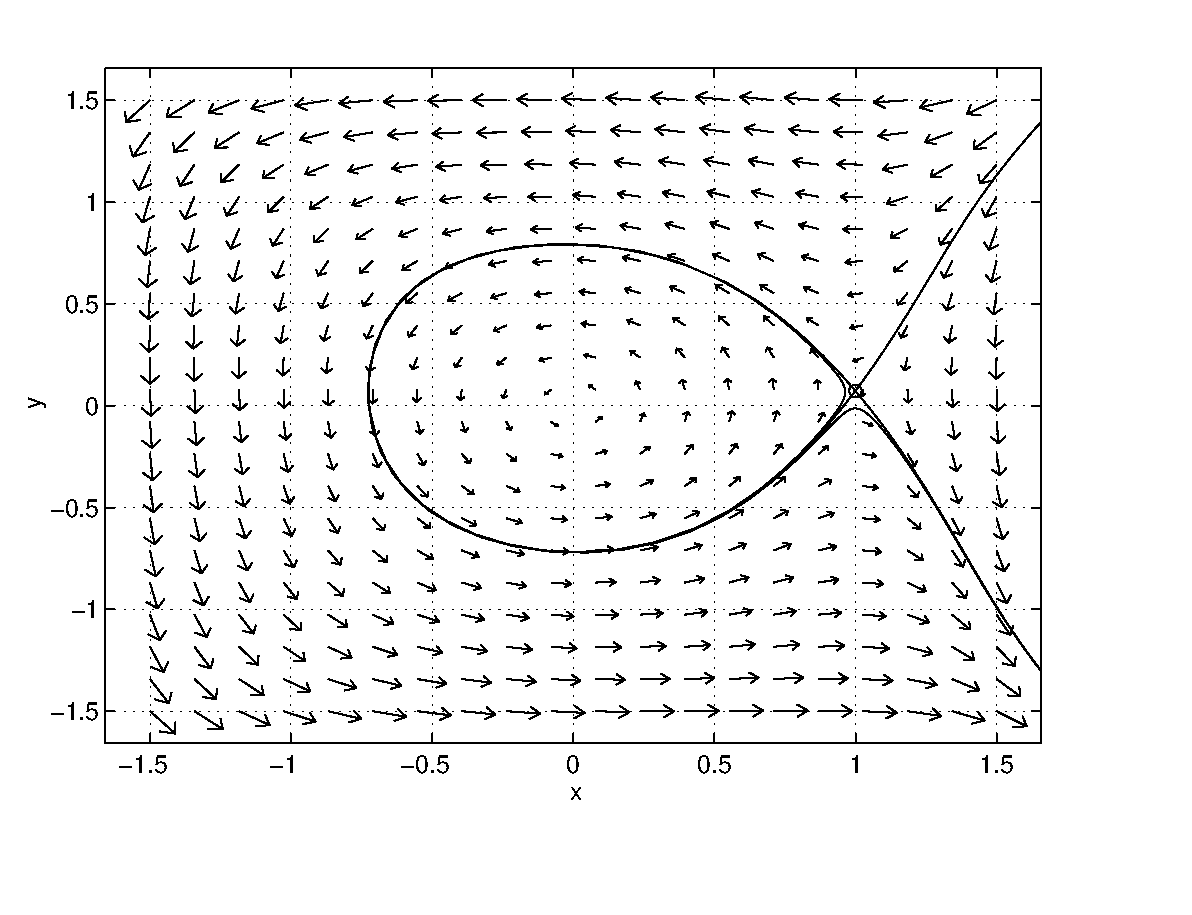
\psfig{file=exfigure/9-6-2c.eps,width=1.8in}}
		\centerline{$\rho = -0.02$\hspace{1.1in}$\rho = -0.03$
\hspace{1.1in}$\rho = -0.027$}
		\centerline{Figure~\ref{c9.6.2a}\hspace{1.2in}
Figure~\ref{c9.6.2b}\hspace{1.2in}Figure~\ref{c9.6.2c}}
\end{figure}

\exer{c9.6.3a}
\ans The system appears to have an infinite number of limit cycles
as the size of the computation area increases.

\soln In the region $-2 \leq x,y \leq 2$, the system appears to have no
limit cycles.  However, in the region $-10 \leq x,y \leq 10$, there are
four limit cycles, and there are more in the larger region $-40 \leq x,y
\leq 40$.  Figure~\ref{c9.6.3a} shows the system with $\rho = 0$ on the
square $-10 \leq x,y \leq 10$.

\exer{c9.6.3b}
Figure~\ref{c9.6.3b}a shows the system with $\rho = 0.06$, and 
Figure~\ref{c9.6.3b}b shows the system with $\rho = 0.07$.  The system
has two periodic solutions at $\rho = 0.06$, and none at $\rho = 0.07$.
A saddle node bifurcation for periodic solutions occurs between these
two values of $\rho$.

\begin{figure}[htb]
                       \centerline{%
                       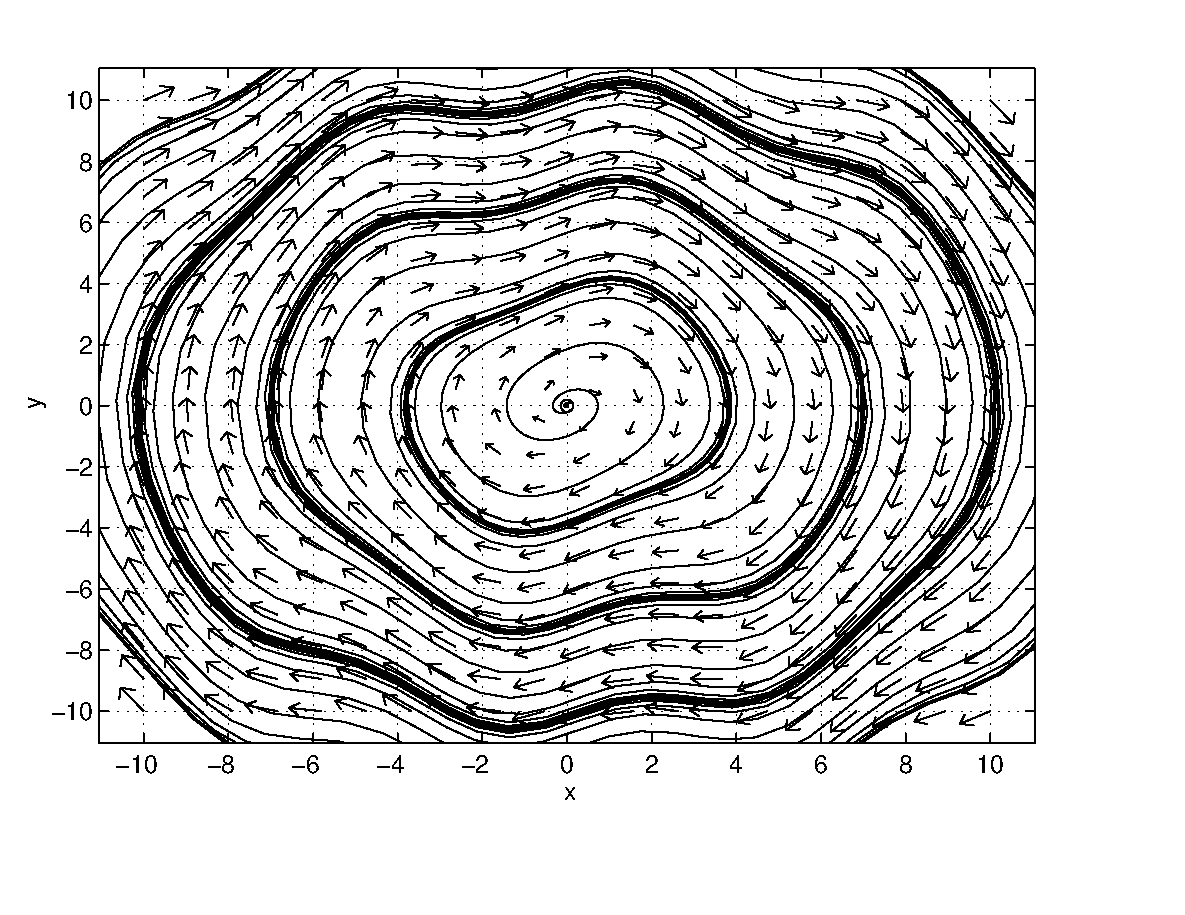
\psfig{file=exfigure/9-6-3a.eps,width=1.8in}
                       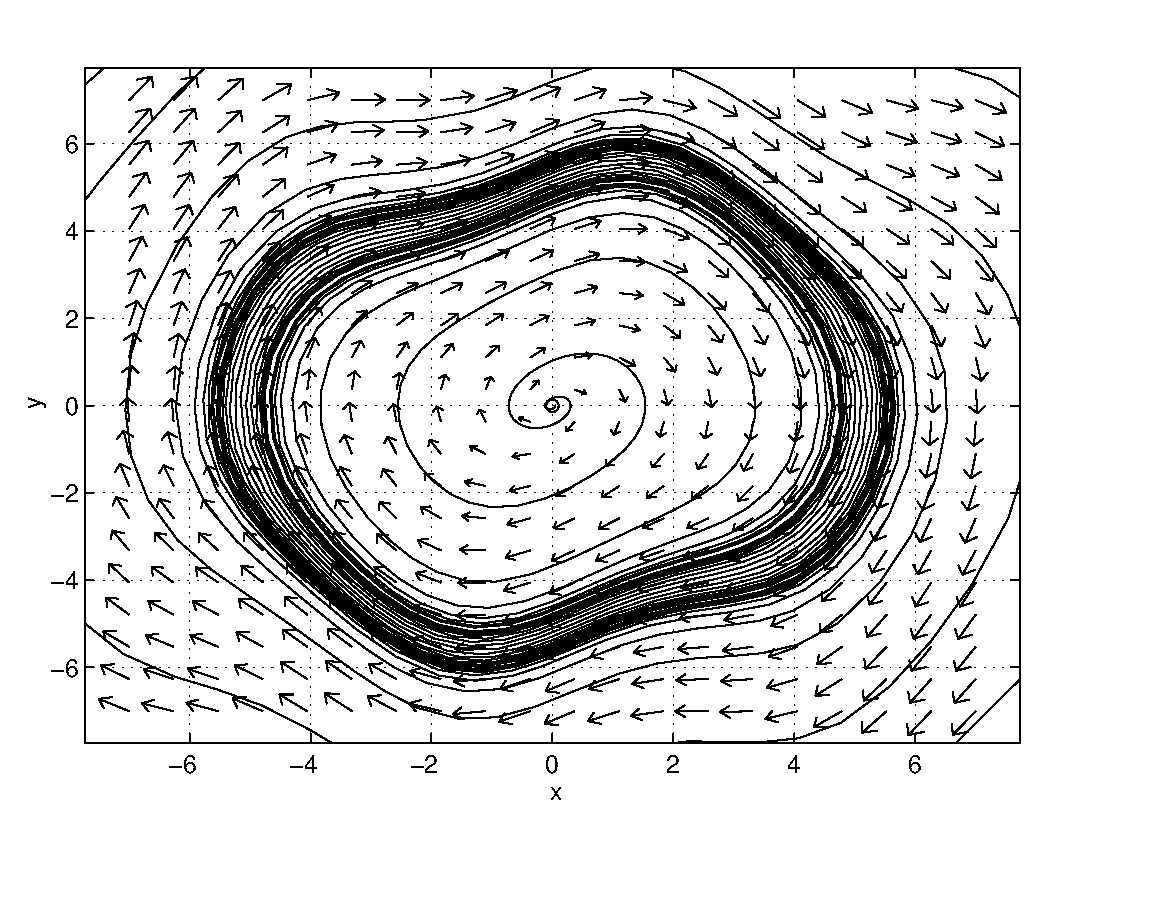
\psfig{file=exfigure/9-6-3b.eps,width=1.8in}
                       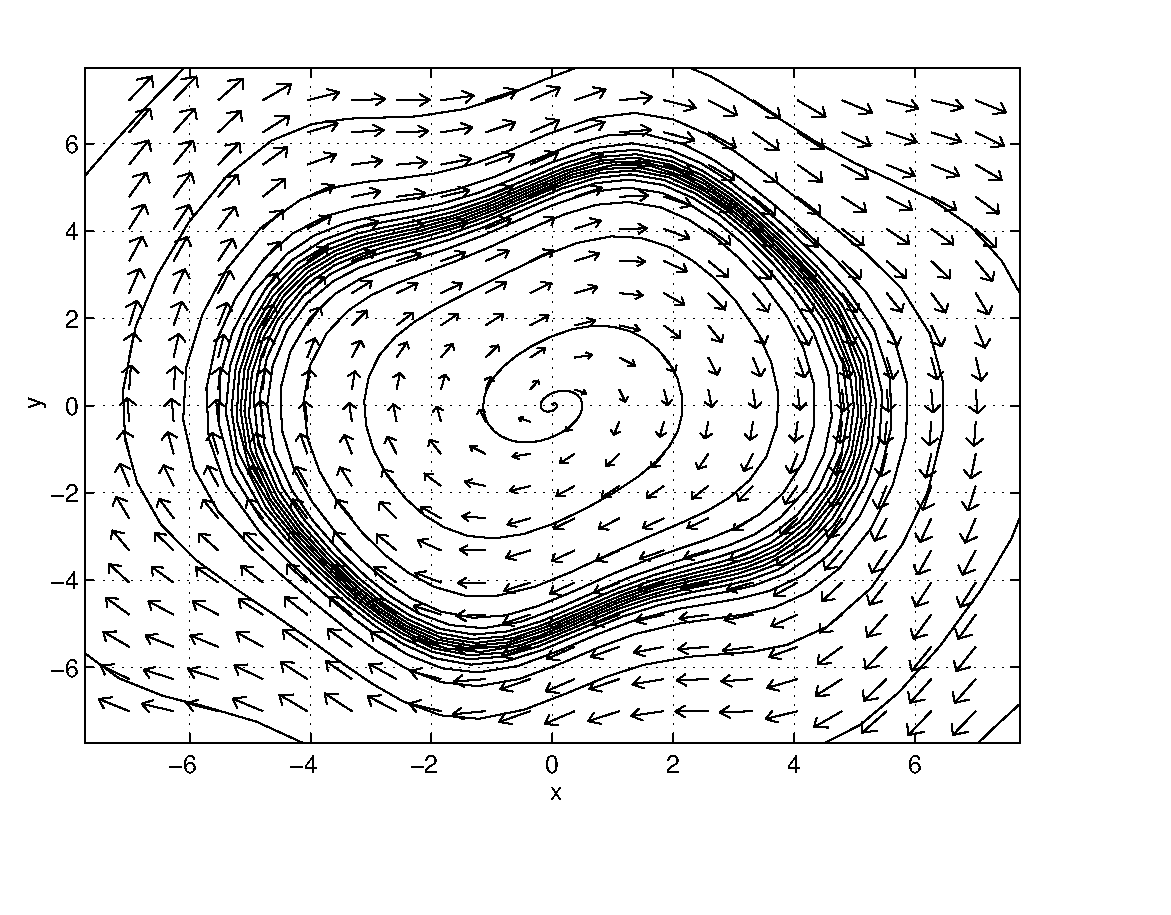
\psfig{file=exfigure/9-6-3c.eps,width=1.8in}}
		\centerline{$\rho = 0$\hspace{1.3in}$\rho = 0.06$
\hspace{1.3in}$\rho = 0.07$}
		\centerline{Figure~\ref{c9.6.3a}\hspace{1.2in}
Figure~\ref{c9.6.3b}a\hspace{1.2in}Figure~\ref{c9.6.3b}b}
\end{figure}

\exer{c9.6.4a}
\ans The system has a saddle at $(x,y) \approx (0.4,-1.2)$, and a 
spiral source at $(x,y) \approx (2.0,1.9)$.

\soln Either determine the equilibria numerically from the {\tt pplane5}
graph of the system (Figure~\ref{c9.6.4b}a), or compute analytically.  To
do this, solve $\dot{y} = 0$ to find that $y = x^3 - 3x$ at all equilibria.
Then, substitute this value for $y$ into $\dot{x}$ and solve $\dot{x} = 0$
to obtain $0 = x^3 + x^2 - 7.4x + 2.89$.  Find the roots of this equation
to confirm that $(x,y) \approx (0.4,-1.2)$ and $(x,y) \approx (2.0,1.9)$
are equilibria.  There is a third equilibrium at $(x,y) \approx
(-3.4,-29)$ which is not in the graph range.

\para The general Jacobian for the system is
\[
J = \cmattwo{-1 + 2(x - \rho)}{1}{-3x^2 + 3}{1}.
\]
Thus, when $\rho = 1.7$, $\trace(J) = 2(x - 1.7)$ and
$\det(J) = 3x^2 + 2(x - 1.7) - 4$.  At $(x,y) \approx (0.4,-1.2)$,
$\det(J) \approx -6.1 < 0$, so the equilibrium is a saddle.  At
$(x,y) \approx (2.0,1.9)$, $\det(J) \approx 8.6 > 0$, $\trace(J) \approx
0.6 > 0$, and $D = (\trace(J))^2 - t\det(J) \approx -34 < 0$.  Therefore,
this equilibrium is a spiral source.

\exer{c9.6.4b} A homoclinic bifurcation occurs between $\rho = 1.7$ and
$\rho = 1.85$.  As $\rho$ increases from $\rho = 1.7$, an unstable
orbit of the saddle point crosses a stable orbit of the saddle.  After
this point, there is a periodic solution around the spiral source.

\exer{c9.6.4c} A Hopf bifurcation occurs between $\rho = 1.85$ and
$\rho = 2.1$.  The spiral source passes through a center and becomes a
spiral sink.  At this point, the periodic solution disappears.

Figure~\ref{c9.6.4b}a shows the system with $\rho = 1.7$.
Figure~\ref{c9.6.4b}b shows the system with $\rho = 1.85$.
Figure~\ref{c9.6.4b}c shows the system with $\rho = 2.1$.

\begin{figure}[htb]
                       \centerline{%
                       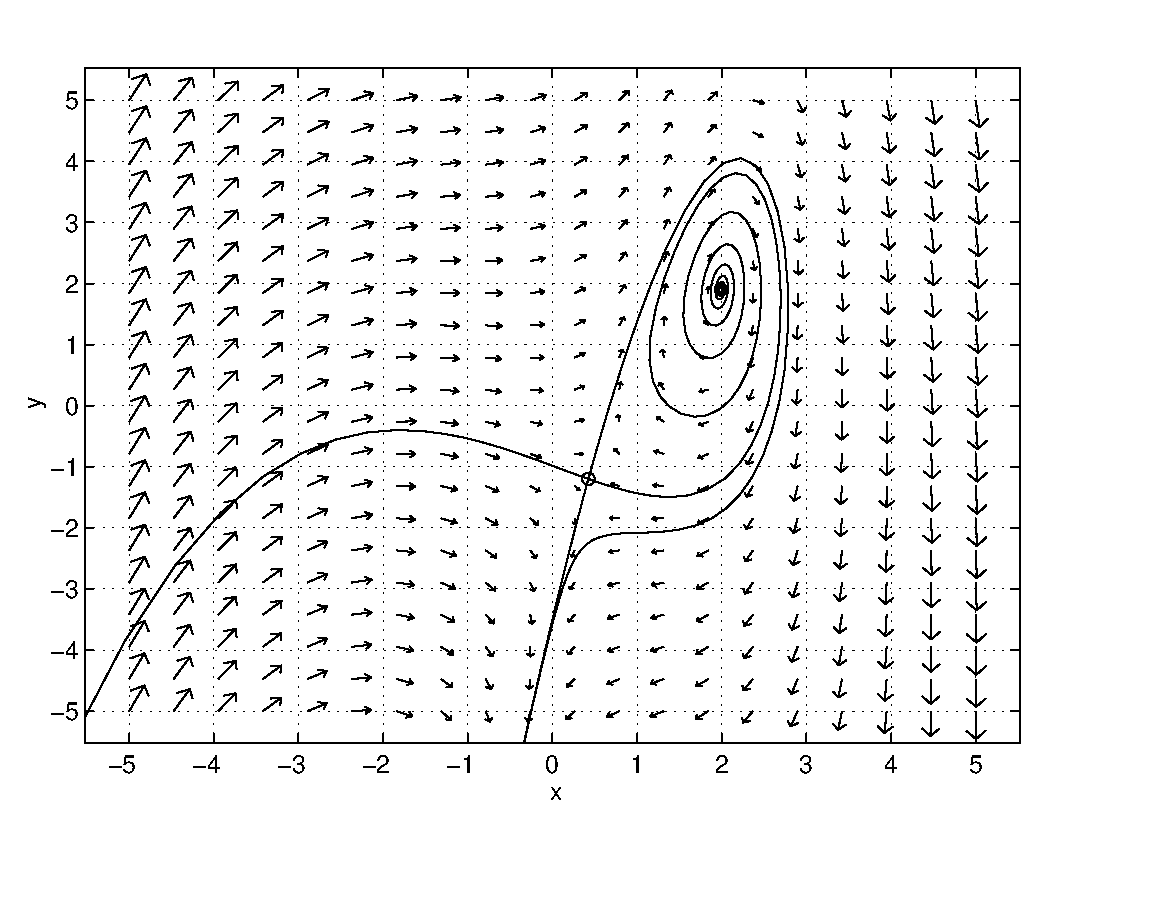
\psfig{file=exfigure/9-6-4a.eps,width=1.8in}
                       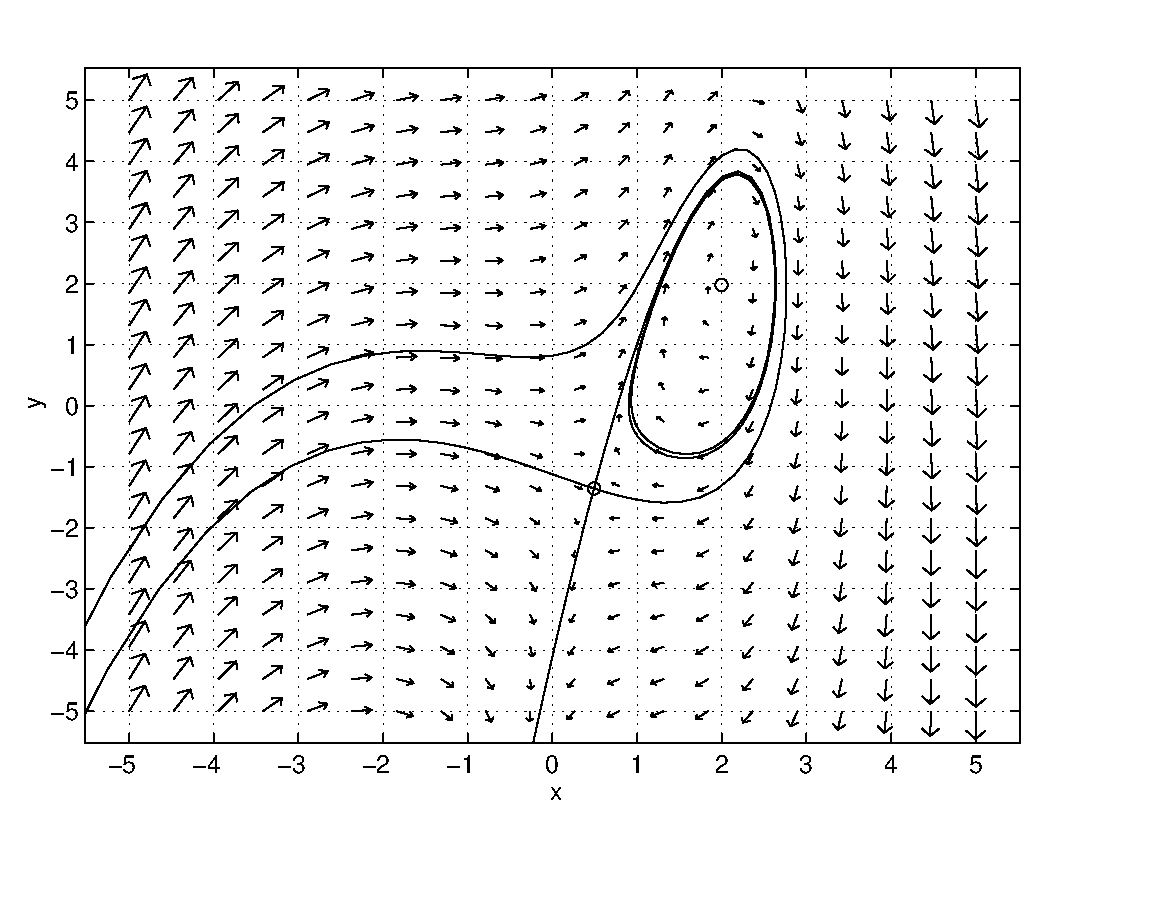
\psfig{file=exfigure/9-6-4b.eps,width=1.8in}
                       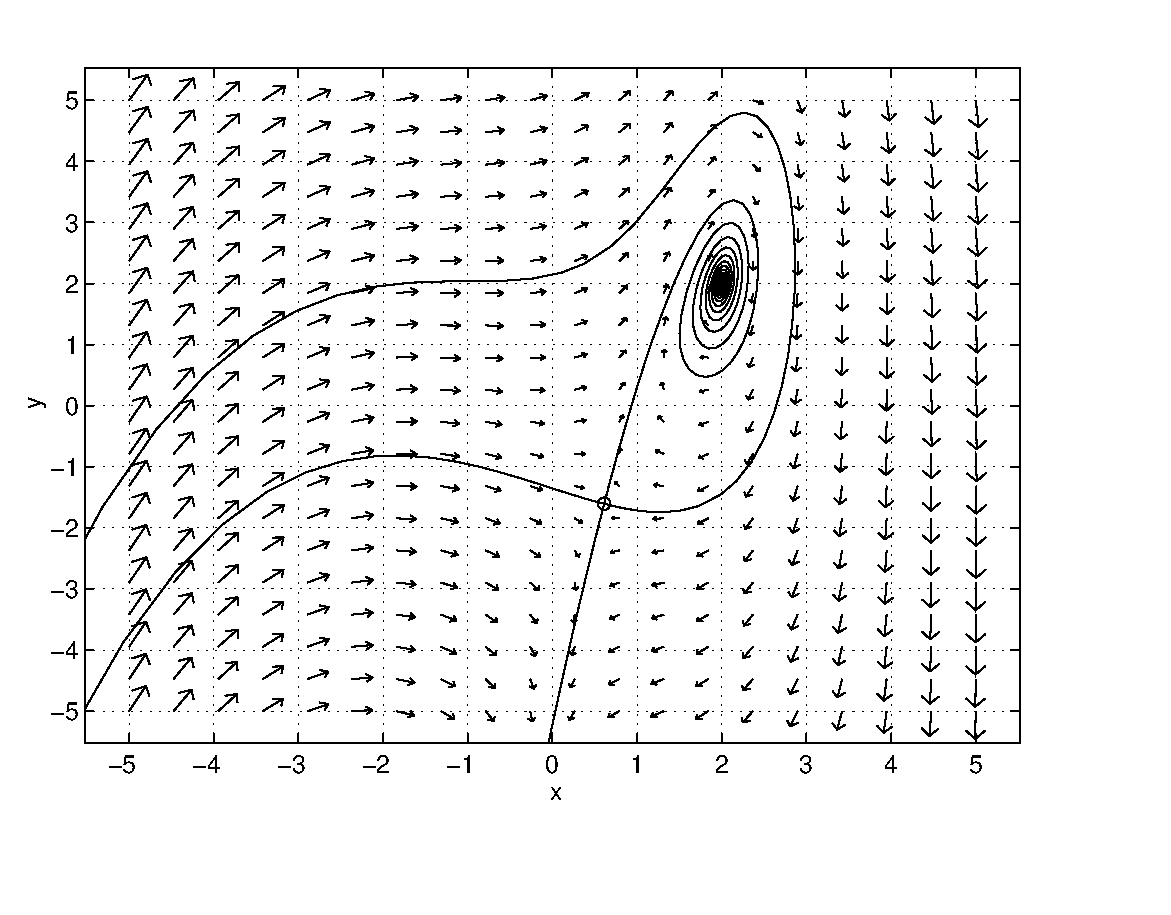
\psfig{file=exfigure/9-6-4c.eps,width=1.8in}}
		\centerline{$\rho = 1.7$\hspace{1.3in}$\rho = 1.85$
\hspace{1.3in}$\rho = 2.1$}
                \exercapthree{c9.6.4b}
\end{figure}


\exer{c9.6.6}
\soln In the family of systems of differential equations  
\[
\begin{array}{rcl}
\dot{x} & = & \rho x-y-3y^2+2.5xy\\
\dot{y} & = & x-3x^2+2x^2y.
\end{array}
\]
there are seven bifurcations as $\rho$ varies from $\rho=-0.1$ to $\rho=0.3$:  
\begin{enumerate}
\item	a saddle-node bifurcation between $\rho=-0.1$ and $\rho=-0.002$,
\item	a Hopf bifurcation between $\rho=-0.002$ and $\rho=0.008$,
\item	a Hopf bifurcation between $\rho=0.008$ and $\rho=0.05$,
\item	a homoclinic bifurcation between $\rho=0.05$ and $\rho=0.08$,
\item	a homoclinic bifurcation between $\rho=0.08$ and $\rho=0.1$,
\item	a heteroclinic bifurcation between $\rho=0.1$ and $\rho=0.2$,
\item	a heteroclinic bifurcation between $\rho=0.2$ and $\rho=0.3$.
\end{enumerate}
The following eight phase portraits bracket the seven bifurcations.
\begin{figure}[htb]
     \centerline{%
     \psfig{file=exfigure/pr3-M1.eps,width=2.75in}     
     \psfig{file=exfigure/pr3-M002.eps,width=2.75in}}
     \centerline{Figure~\ref{c9.6.6}a ($\rho = -0.1$)\hspace{1.3in} Figure~\ref{c9.6.6}b ($\rho = -0.002$)}
\end{figure}
\begin{figure}[htb]
     \centerline{%
     \psfig{file=exfigure/pr3-008.eps,width=2.75in}
     \psfig{file=exfigure/pr3-05.eps,width=2.75in}}
     \centerline{Figure~\ref{c9.6.6}c ($\rho = 0.008$)\hspace{1.3in} Figure~\ref{c9.6.6}d ($\rho = 0.05$)}
\end{figure}
\begin{figure}[htb]
     \centerline{%
     \psfig{file=exfigure/pr3-08.eps,width=2.75in}   
     \psfig{file=exfigure/pr3-1.eps,width=2.75in}}
     \centerline{Figure~\ref{c9.6.6}e ($\rho = 0.08$)\hspace{1.3in} Figure~\ref{c9.6.6}f ($\rho = 0.1$)}
\end{figure}
\begin{figure}[htb]
     \centerline{%
     \psfig{file=exfigure/pr3-2.eps,width=2.75in}     
     \psfig{file=exfigure/pr3-3.eps,width=2.75in}}
     \centerline{Figure~\ref{c9.6.6}g ($\rho = 0.2$)\hspace{1.3in} Figure~\ref{c9.6.6}h ($\rho = 0.3$)}
\end{figure}

\clearpage

\exer{c9.6.5a}
\ans For any values of $\rho$, the system has saddle points at
\[
(x,y) = (-\rho + \sqrt{\rho^2 + 4},0) \AND
(x,y) = (-\rho - \sqrt{\rho^2 + 4},0)
\]
and a spiral sink at the origin.

\soln Set $\dot{x} = \dot{y} = 0$.  Then $y = 0$, and
$0 = x^3 + \rho x^2 - x$, so there are equilibria at the origin, and at
the roots of $x^2 + \rho x - x$.

\exer{c9.6.5b}
One bifurcation occurs as $\rho$ is varied from $\rho = 0.1$ to $\rho = 0.2$.

\exer{c9.6.5c}
A heteroclinic bifurcation occurs at $\rho \approx 0.141$.  At this
point, an unstable orbit of the leftmost saddle point coincides with a
stable orbit of the rightmost saddle point.



\subsection*{Section~\protect{\ref{S:SNB}} Saddle-Node Bifurcations Revisited}
\rhead{S:SNB}{SADDLE-NODE BIFURCATIONS REVISITED}

\exer{c9.3.1}
(a) A steady-state bifurcation occurs on a function $f(x,\rho)$ at a
point $(x,\rho) = (x_0,\rho_0)$ if $f(x_0,\rho_0) = 0$ and
$f_x(x_0,\rho_0) = 0$.  In this case, let $(x_0,\rho_0) = (0,0)$.
Then
\[ \begin{array}{rcccl}
f_1(x_0,\rho_0) & = & \rho_0 - x_0^3 & = & 0 \\
f_{1x}(x_0,\rho_0) & = & -3x_0^2 & = & 0 \end{array}
\qquad
\begin{array}{rcccl}
f_2(x_0,\rho_0) & = & \rho_0x_0 - x_0^2 & = & 0 \\
f_{2x}(x_0,\rho_0) & = & \rho_0 - 2x_0 & = & 0. \end{array}
\]
Therefore, $f_1$ and $f_2$ have steady-state bifurcations at $(x,\rho)
= (0,0)$.

(b) A saddle-node bifurcation occurs on a function $f(x,\rho)$ at a point
$(x,\rho) = (x_0,\rho_0)$ if $f$ has a steady-state bifurcation at this
point, and if $f_\rho(x_0,\rho_0) \neq 0$ and $f_{xx}(x_0,\rho_0) \neq 0$.
Let $(x_0,\rho_0) = (0,0)$.  Then
\[
f_{1xx}(x_0,\rho_0) = -6x = 0 \AND
f_{2p}(x_0,\rho_0) = x = 0,
\]
so neither $f_1$ nor $f_2$ has a saddle-node bifurcation at $x = 0$.

(c) The bifurcation diagram for $f_1$ is shown in Figure~\ref{c9.3.1}a, and
the diagram for $f_2$ is shown in Figure~\ref{c9.3.1}b.  Saddle-node
bifurcations occur only when equilibria appear or disappear.
Figure~\ref{c9.3.1}a shows that $f_1$ has one equilibrium for all $\rho$,
and Figure~\ref{c9.3.1}b shows that $f_2$ has two equilibria for all
$\rho$.  Thus, neither function has a saddle-node bifurcation at the origin.


\begin{figure}[htb]
                       \centerline{%
                       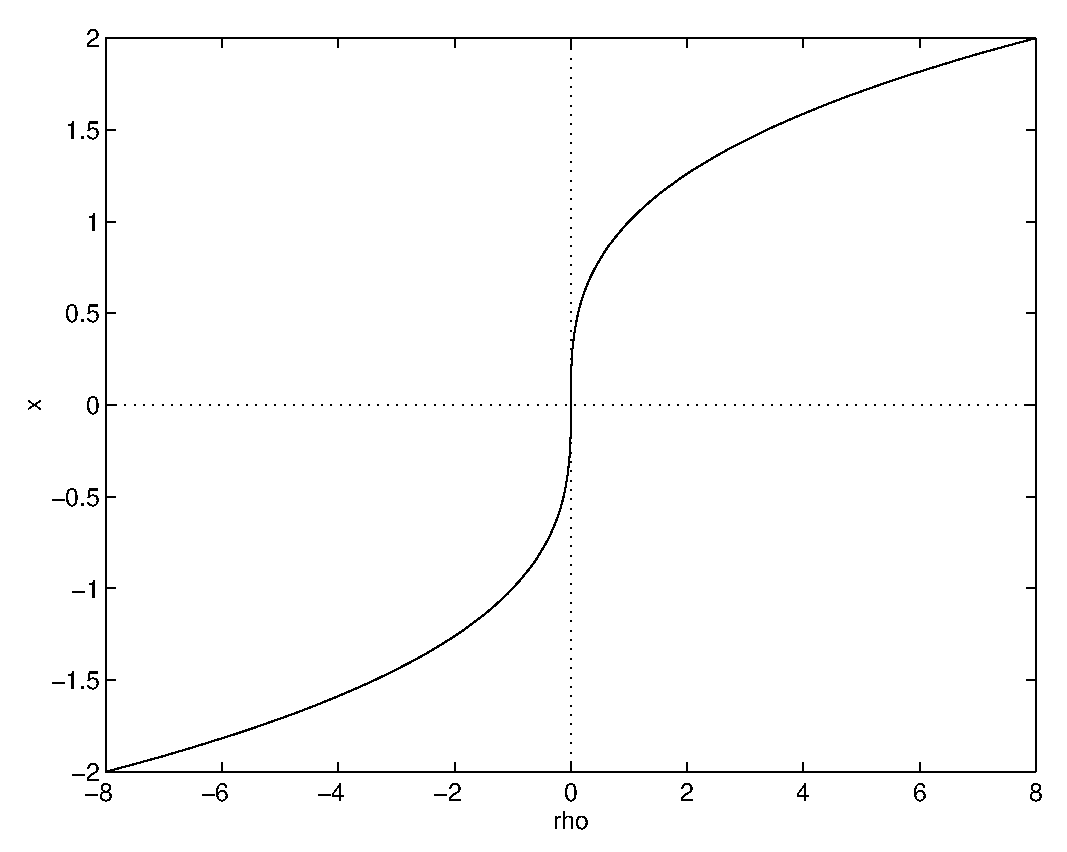
\psfig{file=exfigure/9-3-1a.eps,width=2.75in}
                       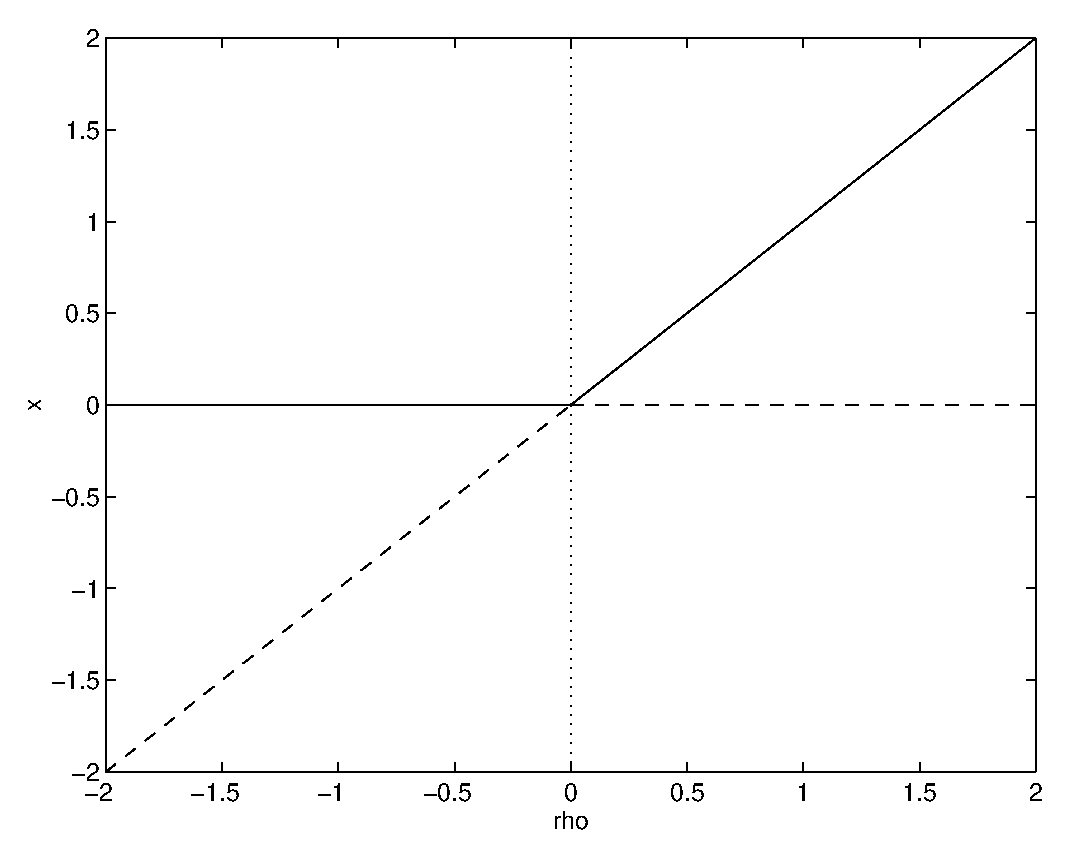
\psfig{file=exfigure/9-3-1b.eps,width=2.75in}}
                \exercaptwo{c9.3.1}
\end{figure}

\exer{c9.3.5}
\ans Saddle-node bifurcations occur at $(x,\rho)=(3,9)$ and 
$(x,\rho)=(1/3,-13/27)$.

\soln A saddle-node bifurcation can occur only at points where
\[ 
f(x,\rho)=0 \quad \mbox{and}\quad f_x(x,\rho)=0,
\]
that is, 
\[
x^3 -5x^2 + 3x + \rho = 0 \AND 3x^2 -10x +3 = (3x-1)(x-3)=0.
\]
From these equations we see that saddle-nodes can occur only at 
$(x,\rho)=(3,9)$ and at $(x,\rho)=(1/3,-13/27)$. Such points are saddle-nodes 
if, in addition, 
\[
f_\rho(x,\rho)\neq 0 \AND  f_{xx}(x,\rho)\neq 0.
\]
Note that
\[
f_\rho(x,\rho) = 1  \AND  f_{xx}(x,\rho) = 6x - 10.
\]
So $f_\rho$ is never zero and $f_{xx}$ is nonzero when $x=3$ and $x=1/3$.
So there are two saddle-node bifurcations.  The 
bifurcation diagram is shown in Figure~\ref{c9.3.5}.
\begin{figure}[htb]
     \centerline{%
     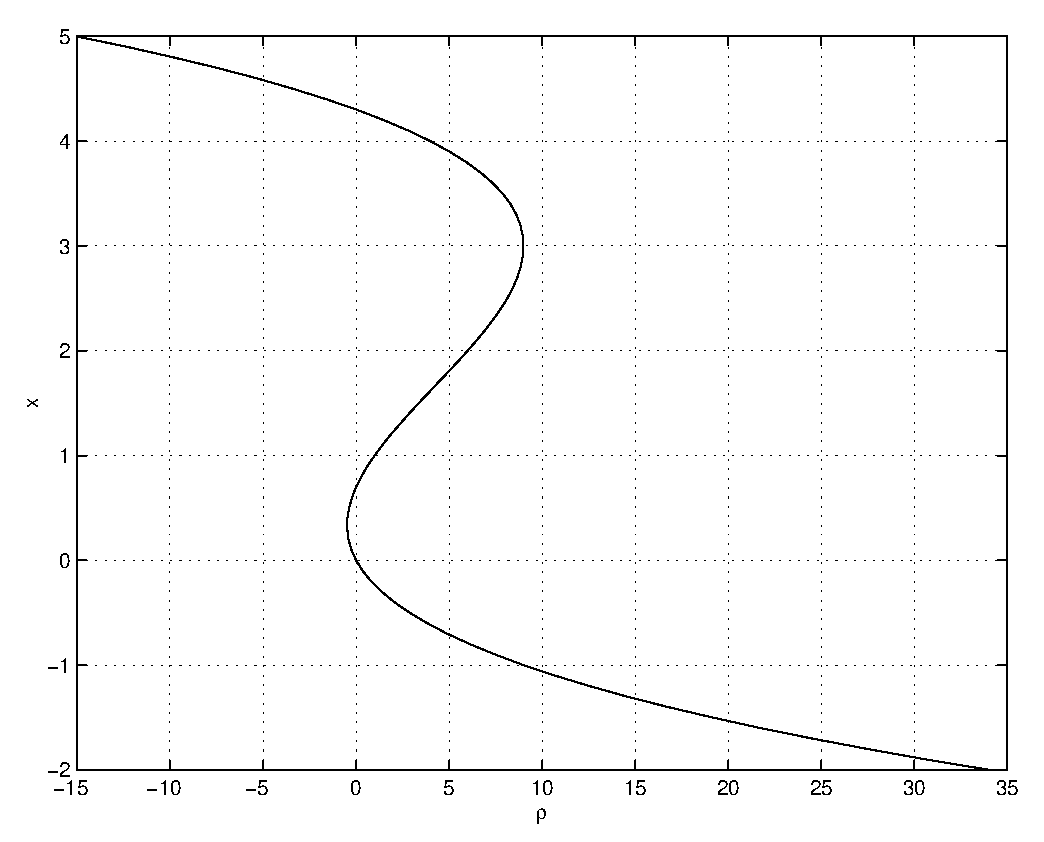
\psfig{file=exfigure/bifdiagex.eps,width=3.0in}}
     \exercap{c9.3.5}
\end{figure}




\exer{c9.3.2}
\ans There are two equilibria near $x = 3$ when $\rho > 1$.

\soln Calculate
\[
f(3,1) = 0, \quad
f_x(3,1) = 0, \quad
f_\rho(3,1) = -6 \neq 0, \AND
f_{xx}(3,1) = 16 \neq 0.
\]
Therefore, $f$ has a saddle-node bifurcation at $x = 3$ when $\rho =
1$.  Note that Theorem~\ref{T:saddlenode} states
that if $a < 0$, then there are two equilibria near $x_0$ for $\rho >
\rho_0$.  In this case,
\[
a = \frac{f_{xx}(x_0,\rho_0)}{f_p(x_0,\rho_0)} = -\frac{8}{3} < 0.
\]

\exer{c9.3.3}
The function $F$ has a bifurcation point at the origin when $\rho = 0$
if $F$ is in equilibrium at $(x,y,\rho) = (0,0,0)$ and $\det(F) = 0$ at
this point.  Since $g(0,0,0) = 0$ and $h(0,0,0) = 0$, the origin is an
equilibrium for $F$ when $\rho = 0$.  Then, calculate the Jacobian at
this point:
\[
J = \mattwo{-2}{1}{4}{-2}.
\]
The determinant of the Jacobian is zero so the origin is indeed a
bifurcation point when $\rho = 0$.  In order to demonstrate the
two-dimensional nondegeneracy conditions, find nonzero vectors $v$ and
$w$ such that $Jv = 0$ and $J^tw = 0$.  In this case, $v = (1,2)^t$ and
$w = (2,1)^t$.  Then, compute
\[
w \cdot F_\rho(0,0,0) = \vectwo{2}{1} \cdot \vectwo{1}{2} =
4 \neq 0,
\]
so \Ref{e:2deig} is satisfied.  In order to satisfy \Ref{e:2dbifur},
compute
\[
g_{xx} = 4, \quad
g_{xy} = 0, \quad
g_{yy} = -6y, \quad
h_{xx} = 0, \quad
h_{xy} = -1, \quad
h_{yy} = 2.
\]
and evaluate
\[
F_0 = \vectwo{4}{0} + 4\vectwo{0}{-1} + 4\vectwo{0}{2} =
\vectwo{4}{1}.
\]
Then, since $w \cdot F_0 = 9 \neq 0$, the second nondegeneracy condition
is satisfied, and the origin is indeed a saddle node bifurcation for $F$
when $\rho = 0$.

\exer{c9.3.4}
To show that the origin is a bifurcation point of $F$ when $\rho = 0$, we
must show the following:

(a) $F(0,0) = 0$.

(b) Let $J = dF_{(0,0)}$.  Then $\det(J) = 0$ and $\trace(J) \neq 0$.

(c) There exist nonzero vectors $v$ and $w$ such that $Jv = 0$ and
$J^tw = 0$.

\soln Let
\[
\vectwo{g(X,\rho)}{h(X,\rho)} = F(X,\rho) = 
\cvectwo{\rho q_1 + x + \alpha x^2 + \beta xy + \gamma y^2}
{\rho q_2 + \delta x^2 + \epsilon xy + \varphi y^2}.
\]

(a) Indeed, $g(0,0) = 0 = h(0,0)$, so $F(0,0)$ is an equilibrium point.

(b) Find the Jacobian
\[
J = \left.\cmattwo{1 + 2\alpha x + \beta y}{\beta x + 2\gamma y}
{2\delta x + \epsilon y}{\epsilon x + 2\varphi y}\right|_{(0,0)} =
\mattwo{1}{0}{0}{0}.
\]
Since $\det(J) = 0$ and $\trace(J) = 1 \neq 0$, there
is a bifurcation point at the origin with $\rho = 0$.

(c)  To verify that the nondegeneracy conditions are satisfied, find $v$
and $w$.  In this case $v = w = (0,1)^t$.  Then verify
\[
w \cdot F_\rho(X_0,\rho_0) = \vectwo{0}{1} \cdot \vectwo{q_1}{q_2}
= q_2.
\]
So, condition \Ref{e:2deig} is satisfied when $q_2 \neq 0$.  To
verify \Ref{e:2dbifur}, compute the vector
\[
F_0 = 0\vectwo{g_{xx}}{h_{xx}} + 0\vectwo{g_{xy}}{h_{xy}} +
\vectwo{g_{yy}}{h_{yy}} = \vectwo{2\gamma}{2\varphi}
\]
and calculate
\[
w \cdot F_0 = \vectwo{0}{1} \cdot \vectwo{2\gamma}{2\varphi}
= 2\varphi.
\]
So, the origin is a saddle node of $F$ with $\rho = 0$ when
$q_2 \neq 0$ and $\varphi \neq 0$.



\subsection*{Section~\protect{\ref{S:HopfBif}} *Hopf Bifurcations Revisited}
\rhead{S:HopfBif}{*HOPF BIFURCATIONS REVISITED}


\exer{c9.6.1a}
\ans The only equilibria of this system occur at the origin and a point of
Hopf bifurcation occurs at $\rho=0$.  The eigenvalue crossing condition is
satisfied.

\soln  To find the equilibria solve $\dot{y}=0$ for $x=0$ and $\dot{x}=0$ for
$y=0$.  The Jacobian matrix at the origin is 
\[
J(\rho) = \mattwo{\rho}{-1}{1}{0}.
\]
Thus, $\trace(J(\rho))=0$ only when $\rho=0$.  So a Hopf bifurcation point
can only occur at $\rho=0$.  Finally, note that 
\[
\frac{d}{dt}\trace(J(\rho)) = 1 \neq 0;
\]
So the eigenvalue crossing condition is satisfied.


\exer{c9.6.1b}
\ans  There are two possible points of Hopf bifurcation: one at $(0,0)$ 
when $\rho=0$ and $(1,0)$ at $\rho=-1$.  The eigenvalue crossing condition is
satisfied at both points.

\soln  The system of differential equations
\[
\begin{array}{rcl}
\dot{x} & = & y - \rho x - x^2   \\
\dot{y} & = & -x - \rho y + x^2.
\end{array}
\]
has Jacobian matrix 
\[
J = \cmattwo{-\rho-2x}{1}{-1+2x}{-\rho}.
\]
Since a point of Hopf bifurcation must be at an equilibrium where the trace
of the Jacobian matrix is zero, points of Hopf bifurcation must satisfy the
three equations:
\begin{eqnarray*}
y - \rho x - x^2 & = & 0\\
-x - \rho y + x^2 & = & 0\\
-2\rho-2x & = & 0.
\end{eqnarray*}
On substituting $\rho = -x$ into the first two equations, we obtain:
\begin{eqnarray*}
y  & = & 0\\
-x + xy + x^2 & = & 0
\end{eqnarray*}
From these equations we see that there are two possible points of Hopf
bifurcation $(0,0)$ at $\rho=0$ or $(1,0)$ at $\rho=-1$.  

To check the eigenvalue crossing condition we must compute the trace of the
Jacobian matrix along the branch of equilibria.  To find the branches we must
solve the equilibrium equations
\begin{eqnarray*}
y - \rho x - x^2 & = & 0\\
-x - \rho y + x^2 & = & 0
\end{eqnarray*}
for $x$ and $y$ as a function of $\rho$.  Substituting $y - \rho x+x^2$ into
the $2^{nd}$ equation yields:
\[
-(1+\rho^2)x + (1-\rho)x^2 = 0.
\]
Therefore either 
\[
x= 0 \quad \mbox{ or } \quad  x = \frac{1+\rho^2}{1-\rho}.
\]
If $x=0$, then $y=0$ and the trace of the Jacobian along this branch is
$-2\rho$.  Since the derivative with respect to $\rho$ equals $-2$, the
eigenvalue crossing condition is satisfied.

In the second case, the trace of the Jacobian along the branch of equilibria
equals
\[
-2\rho-2x = -2\rho -2\frac{1+\rho^2}{1-\rho}.
\]
The derivative of this expression with respect to $\rho$ is $3$ at $\rho=-1$.
Hence the eigenvalue crossing condition is satisfied.


